\documentclass[11pt,letterpaper,openany]{book}

% Essential packages in correct loading order
\usepackage[T1]{fontenc}
\usepackage[utf8]{inputenc}
\usepackage{lmodern}
\usepackage[margin=1in]{geometry}
\usepackage{microtype}
\usepackage{graphicx}
\usepackage{float}
\usepackage{xcolor}
\usepackage{titlesec}
\usepackage{tocloft}
\usepackage{fancyhdr}
\usepackage{etoc}
\usepackage{booktabs}
\usepackage{tikz}
\usepackage{afterpage}
\usepackage{wrapfig}
\usepackage{tcolorbox}
\usepackage{caption}
\usepackage{amsmath}
\usepackage{listings}
\usepackage{hyperref}
\usepackage[nameinlink]{cleveref}
\usepackage{bookmark}
\usepackage{pgf-pie}  % For pie charts
\usepackage{placeins} % For float placement

% Fix float placement
\makeatletter
\def\fps@figure{htbp}
\makeatother

% Define pie chart colors
\definecolor{piecolor1}{RGB}{51,153,255}
\definecolor{piecolor2}{RGB}{0,102,0}
\definecolor{piecolor3}{RGB}{153,0,0}
\definecolor{piecolor4}{RGB}{255,153,0}

% For better figure placement
\renewcommand{\topfraction}{0.9}
\renewcommand{\bottomfraction}{0.9}
\renewcommand{\textfraction}{0.1}
\renewcommand{\floatpagefraction}{0.7}

% Fix itemize spacing
\usepackage{enumitem}
\setlist[itemize]{topsep=0pt,itemsep=0pt,parsep=0pt,partopsep=0pt}

% Additional TikZ libraries
\usetikzlibrary{arrows.meta}
\usetikzlibrary{backgrounds}
\usetikzlibrary{calc}

% For better table formatting
\usepackage{array}
\usepackage{tabularx}
\usepackage{longtable}

% Fix page breaks
\raggedbottom

% Fix chapter spacing
\titlespacing*{\chapter}{0pt}{-50pt}{40pt}

% TikZ libraries
\usetikzlibrary{arrows,shapes,positioning,shadows,trees}

% Color definitions
\definecolor{primarydark}{RGB}{0,71,187}     % Deep Blue
\definecolor{primary}{RGB}{51,153,255}       % Bright Blue
\definecolor{primarylight}{RGB}{204,229,255} % Light Blue
\definecolor{secondarydark}{RGB}{0,102,0}    % Deep Green
\definecolor{secondary}{RGB}{51,204,51}      % Bright Green
\definecolor{secondarylight}{RGB}{229,255,229} % Light Green
\definecolor{accentdark}{RGB}{153,0,0}       % Deep Red
\definecolor{accent}{RGB}{255,51,51}         % Bright Red
\definecolor{accentlight}{RGB}{255,204,204}  % Light Red

% Chapter and section styling
\titleformat{\chapter}[display]
{\normalfont\huge\bfseries\color{primarydark}}
{\chaptertitlename\ \thechapter}{20pt}{\Huge}

\titleformat{\section}
{\normalfont\Large\bfseries\color{primary}}
{\thesection}{1em}{}

\titleformat{\subsection}
{\normalfont\large\bfseries\color{primarydark}}
{\thesubsection}{1em}{}

% Table of contents styling
\renewcommand{\cftsecleader}{\cftdotfill{\cftdotsep}}
\renewcommand{\cftchapfont}{\color{primarydark}\bfseries}
\renewcommand{\cftsecfont}{\color{primary}}
\renewcommand{\cftsubsecfont}{\color{primarydark}}

% Header and footer styling
\pagestyle{fancy}
\fancyhf{}
\fancyhead[LE,RO]{\thepage}
\fancyhead[LO]{\nouppercase{\rightmark}}
\fancyhead[RE]{\nouppercase{\leftmark}}
\fancyfoot[C]{\textcolor{primary}{\rule{0.5\textwidth}{0.4pt}}}

% Hyperref setup
\hypersetup{
    colorlinks=true,
    linkcolor=primarydark,
    filecolor=accent,
    urlcolor=secondary,
    pdftitle={The Nigerian Business Opportunity Blueprint},
    pdfauthor={Dele Omotosho, Counseal},
    pdfsubject={Nigerian Market Entry Guide},
    pdfkeywords={Nigeria, Business, Market Entry, Diaspora, Investment},
}

% Custom box styles
\newtcolorbox{warningbox}{
    colback=accentlight,
    colframe=accentdark,
    title=Warning,
    fonttitle=\bfseries
}

\newtcolorbox{importantbox}{
    colback=secondarylight,
    colframe=secondarydark,
    title=Important,
    fonttitle=\bfseries
}

\newtcolorbox{regionalbox}{
    colback=primarylight,
    colframe=primarydark,
    title=Regional Insight,
    fonttitle=\bfseries
}

\newtcolorbox{workshopbox}{
    colback=white,
    colframe=primary,
    title=Chapter Workshop,
    fonttitle=\bfseries
}

\newtcolorbox{communitybox}{
    colback=secondarylight,
    colframe=secondary,
    title=Africa Growth Circle Community,
    fonttitle=\bfseries
}

% Listing style
\lstset{
    basicstyle=\ttfamily\small,
    breaklines=true,
    commentstyle=\color{accentdark},
    keywordstyle=\color{primarydark},
    stringstyle=\color{secondary},
    numbers=left,
    numberstyle=\tiny\color{primary},
    numbersep=5pt,
    frame=single,
    framesep=5pt,
    rulecolor=\color{primary},
}

% Caption style
\DeclareCaptionFont{primarydarkcolor}{\color{primarydark}}
\captionsetup{
    font=small,
    labelfont={primarydarkcolor,bf},
    margin=10pt
}

% Set headheight
\setlength{\headheight}{14pt}

% Define current date command
\newcommand{\currentdate}{\today}

\begin{document}

    \frontmatter

    \begin{titlepage}
        \centering
        \vspace*{2cm}
        {\Huge\bfseries\color{primarydark} The Nigerian Business\\Opportunity Blueprint\par}
        \vspace{1cm}
        {\Large\color{primary} Your Global Guide to Nigerian Market Entry\par}
        \vspace{2cm}
        {\Large\itshape Dele Omotosho, Counseal.com\par}
        \vspace{1cm}
        {\large Empowering Nigerian Dreams Through Global Access\par}
        \vfill
        {\large Join the Africa Growth Circle Community at circle.counseal.com\par}
        \vspace{1cm}
        {\large \currentdate\par}
    \end{titlepage}

    \tableofcontents

    \mainmatter

    % chapters/00-introduction.tex

\chapter*{Your Journey to Nigerian Market Entry}

\section{Why Nigeria, Why Now}
Nigeria stands at the crossroads of unprecedented opportunity...

\section{How to Use This Book}

\begin{importantbox}
This book is designed to be both a comprehensive guide and a practical workbook. Each chapter builds upon the previous one while remaining independently valuable for your specific needs.
\end{importantbox}

\subsection{Navigation Guide}
\begin{itemize}
    \item \textbf{Regional Insights:} Look for regional boxes highlighting specific considerations for your market
    \item \textbf{Workshops:} Each chapter ends with practical exercises
    \item \textbf{Community Integration:} Links to additional resources in the Africa Growth Circle
\end{itemize}

\section{Quick Assessment: Is Nigerian Market Entry Right for You?}

\begin{workshopbox}
\textbf{Market Entry Readiness Assessment}

Rate your readiness in each area (1-5):
\begin{itemize}
    \item Market Knowledge: \_\_\_
    \item Financial Readiness: \_\_\_
    \item Time Commitment: \_\_\_
    \item Risk Tolerance: \_\_\_
    \item Local Network: \_\_\_
\end{itemize}

Total your score and refer to the interpretation guide on page XX.
\end{workshopbox}

\section{Reading Pathways Based on Your Region}

\begin{regionalbox}{United Kingdom Focus}
Priority chapters for UK-based financial services professionals:
\begin{itemize}
    \item Chapter 2: Entry Strategy (Financial Services Framework)
    \item Chapter 5: Financial Planning (UK Investment Structures)
    \item Chapter 7: Local Network (Financial Services Networks)
\end{itemize}
\end{regionalbox}

\begin{regionalbox}{United States Focus}
Priority chapters for US-based tech entrepreneurs:
\begin{itemize}
    \item Chapter 2: Entry Strategy (Tech Startup Framework)
    \item Chapter 8: Technology Operations
    \item Chapter 9: Growth and Scaling
\end{itemize}
\end{regionalbox}

\begin{regionalbox}{UAE Focus}
Priority chapters for UAE-based trade specialists:
\begin{itemize}
    \item Chapter 2: Entry Strategy (Trade License Framework)
    \item Chapter 6: Risk Management (Trade Compliance)
    \item Chapter 7: Local Network (Trade Associations)
\end{itemize}
\end{regionalbox}

\begin{regionalbox}{Canadian Focus}
Priority chapters for Canadian-based professionals:
\begin{itemize}
    \item Chapter 2: Entry Strategy (Sector-Specific Requirements)
    \item Chapter 5: Financial Planning (Sector-Specific Grants)
    \item Chapter 8: Technology Operations (Industry Solutions)
\end{itemize}
\end{regionalbox}

\section{Accessing the Africa Growth Circle Community}

\begin{communitybox}
Your book purchase includes access to our exclusive community at circle.counseal.com
\begin{itemize}
    \item Access extended case studies
    \item Connect with fellow entrepreneurs
    \item Join regional discussion groups
    \item Access digital templates and tools
    \item Participate in expert office hours
\end{itemize}
\end{communitybox}

\begin{warningbox}
While this book provides comprehensive guidance, always consult with qualified professionals for legal, tax, and regulatory matters specific to your situation.
\end{warningbox}

% End of chapter workshop
\begin{workshopbox}
\textbf{Chapter 0 Action Items}
\begin{itemize}
    \item Complete the Market Entry Readiness Assessment
    \item Identify your regional priority chapters
    \item Set up your Africa Growth Circle account
    \item Connect with your regional discussion group
    \item Download the digital resources for Chapter 1
\end{itemize}
\end{workshopbox}
    \chapter{Understanding the Nigerian Business Landscape}\label{ch:understanding-the-nigerian-business-landscape}

\begin{importantbox}
This chapter provides a clear, practical understanding of Nigeria's business environment, focusing on what truly matters for your success and backed by real market insights.
\end{importantbox}

\section{The Real Nigeria: Beyond the Headlines}\label{sec:the-real-nigeria:-beyond-the-headlines}

I remember sitting in a Boston coffee shop in 2015, meeting with a potential investor interested in Nigerian tech opportunities.\ As he stirred his cappuccino, he said something that still resonates: ``Dele, isn't it too risky?
I mean, with all the\ldots'' He trailed off, gesturing vaguely at imagined chaos.

Several weeks later, I watched that same investor standing in Victoria Island, Lagos, completely transformed.\ ``This isn't anything like what I expected,'' he admitted, watching streams of young professionals heading to their fintech jobs, banks, and digital agencies.\ ``Why doesn't anyone show this side of Nigeria?''

This disconnect between perception and reality is something I've encountered countless times in my journey from Boston's tech scene to building Counseal.
Let's address some common misconceptions with real-world context:

\begin{center}
\begin{tabularx}{\textwidth}{>{\raggedright\arraybackslash}X >{\raggedright\arraybackslash}X}
    \toprule
    \textbf{Common Perception} & \textbf{Market Reality} \\
    \midrule
    ``Everything moves too slowly'' & While some processes take time, well-prepared companies often complete market entry in under 3 months.\ The key is understanding which processes can be parallel-tracked. \\
    \addlinespace
    ``You need political connections'' & Most successful entrepreneurs I work with succeed through standard business practices and professional networks, not political ties. \\
    \addlinespace
    ``Technology infrastructure is poor'' & Lagos's tech infrastructure rivals many global cities.\ Multiple successful fintech companies process millions of transactions daily. \\
    \addlinespace
    ``Too much corruption'' & Clear compliance processes exist.\ Companies regularly succeed without compromising their values through proper documentation and procedures. \\
    \bottomrule
\end{tabularx}
\end{center}

\section{Market Dynamics: The Three Forces}\label{sec:market-dynamics:-the-three-forces}

Think of Nigeria's market as a powerful river system, where three main currents create unique opportunities:

\subsection{The Scale Advantage}\label{subsec:the-scale-advantage}
When a Canadian agritech company wanted to expand here, their initial pilot with 100 farmers quickly scaled to 1,000.\ Why?
Because in Nigeria, word of mouth travels fast in connected communities.\ The same infrastructure investment that serves 100 can often serve 1,000 with minimal additional cost.

\begin{tcolorbox}[colback=white,colframe=primarydark,title=\textbf{Scale Impact Examples}]
\begin{itemize}
    \item A payment solution reaching 1 million users within 6 months of launch
    \item An educational platform scaling from 500 to 5,000 students in one academic year,
    \item A logistics solution expanding from 3 to 15 cities using the same core infrastructure
\end{itemize}
\end{tcolorbox}

\subsection{The Innovation Appetite}\label{subsec:the-innovation-appetite}
Contrary to common belief, Nigerians are early adopters of innovative solutions.\ A UK fintech founder was surprised when their new payment solution gained traction faster in Lagos than in London.\ The reason?
Nigerians actively seek better solutions to existing challenges.

\begin{tcolorbox}[colback=white,colframe=primary,title=\textbf{Innovation Adoption Examples}]
\begin{itemize}
    \item Mobile money adoption rate exceeding many developed markets
    \item Rapid uptake of digital banking solutions
    \item Quick adaptation to e-commerce platforms
\end{itemize}
\end{tcolorbox}

\subsection{The Adaptation Advantage}\label{subsec:the-adaptation-advantage}
Those who succeed here learn to turn challenges into opportunities.\ One UAE founder entered during a foreign exchange restriction period.\ Instead of retreating, they built a local supplier network that now gives them a competitive edge, even after restrictions eased.

\section{Understanding Nigerian Business Culture}\label{sec:understanding-nigerian-business-culture}

Nigerian business culture rests on what I call the ``Three R's'': Relationships, Respect, and Reciprocity.\ Understanding these principles is crucial for success:

\begin{tcolorbox}[colback=white,colframe=primarydark,title=\textbf{The Three R's of Nigerian Business}]
\begin{itemize}
    \item \textbf{Relationships:} Business here is personal.\ Build relationships before transactions.
    \item \textbf{Respect:} Age, experience, and position matter significantly.\ Show appropriate respect in meetings and negotiations.
    \item \textbf{Reciprocity:}  Build mutual benefit into your business relationships.
\end{itemize}
\end{tcolorbox}

\section{High-Potential Sectors}\label{sec:high-potential-sectors}

Based on current market trends and opportunities, these sectors show particular promise:

\begin{tcolorbox}[colback=white,colframe=primary,title=\textbf{Growth Sectors}]
\begin{itemize}
    \item \textbf{Financial Services \& Fintech:}
    Growing at unprecedented rates with regular new entrants.\ Key opportunities in payment solutions, lending platforms, and wealth management.

    \item \textbf{Agriculture \& AgriTech:}
    Massive modernization opportunity, particularly in supply chain optimization, farmer financing, and precision farming.

    \item \textbf{E-commerce \& Logistics:}
    Rapidly evolving with urban growth.\ Opportunities in last-mile delivery, warehouse automation, and digital marketplaces.

    \item \textbf{Education Technology:}
    Huge demand with growing middle class.\ Focus areas include professional development, vocational training, and K-12 supplementary education.

    \item \textbf{Healthcare Innovation:}
    Untapped potential for tech solutions in telemedicine, health records management, and pharmaceutical supply chains.
\end{itemize}
\end{tcolorbox}

\section{Market Entry Workshop}\label{sec:market-entry-workshop}

\begin{workshopbox}
\textbf{Chapter 1 Application Exercise}

1. Misconception Analysis
\begin{itemize}
    \item List your top three concerns about the Nigerian market: \_\_\_\_\_\_\_\_\_
    \item Research-based reality for each concern: \_\_\_\_\_\_\_\_\_
    \item Action plan to address each: \_\_\_\_\_\_\_\_\_
\end{itemize}

2. Sector Opportunity Assessment
\begin{itemize}
    \item Primary sector of interest: \_\_\_\_\_\_\_\_\_
    \item Key opportunities identified: \_\_\_\_\_\_\_\_\_
    \item Potential challenges: \_\_\_\_\_\_\_\_\_
    \item Initial action steps: \_\_\_\_\_\_\_\_\_
\end{itemize}

3. Cultural Adaptation Plan
\begin{itemize}
    \item Key relationship-building activities: \_\_\_\_\_\_\_\_\_
    \item Respect protocols to implement: \_\_\_\_\_\_\_\_\_
    \item Reciprocity opportunities: \_\_\_\_\_\_\_\_\_
\end{itemize}
\end{workshopbox}

\begin{communitybox}
Access additional resources and connect with fellow entrepreneurs on the Africa Growth Circle:
\begin{itemize}
    \item Detailed sector reports
    \item Cultural navigation guides
    \item Expert office hours
    \item Peer networking events
\end{itemize}
Visit \href{https://viz.li/csl-book-circle}{circle.counseal.com} to join the conversation.
\end{communitybox}

\begin{importantbox}
In Chapter 2, we'll build on this foundation to develop your specific entry strategy, including detailed planning frameworks and implementation guides tailored to your sector.
\end{importantbox}
    % chapters/02-entry-strategy.tex

\chapter{Building Your Entry Strategy}

\begin{importantbox}
This chapter provides a structured approach to developing your market entry strategy, with specific frameworks for different business types and regions. The tools and templates provided can be customized to your specific needs.
\end{importantbox}

\section{Choosing Your Market Entry Model}

\subsection{Entry Models Overview}
\begin{center}
\begin{tabular}{p{0.2\textwidth}|p{0.25\textwidth}|p{0.25\textwidth}|p{0.2\textwidth}}
    \textbf{Model} & \textbf{Advantages} & \textbf{Challenges} & \textbf{Best For} \\
    \hline
    Direct Entry & Full control & Higher resource needs & Established firms \\
    Partnership & Local knowledge & Shared control & New entrants \\
    Acquisition & Quick entry & Higher initial cost & Strategic buyers \\
    Representative & Lower risk & Limited control & Market testing \\
\end{tabular}
\end{center}

\subsection{Decision Framework}
\begin{figure}[h]
    \centering
    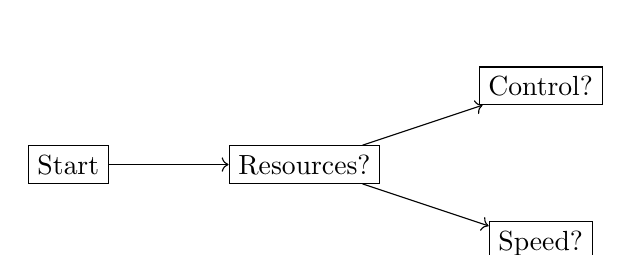
\begin{tikzpicture}
        % Decision tree for entry model selection
        \node[draw] (start) at (0,0) {Start};
        \node[draw] (resources) at (3,0) {Resources?};
        \node[draw] (control) at (6,1) {Control?};
        \node[draw] (speed) at (6,-1) {Speed?};

        \draw[->] (start) -- (resources);
        \draw[->] (resources) -- (control);
        \draw[->] (resources) -- (speed);
    \end{tikzpicture}
    \caption{Entry Model Decision Tree}
\end{figure}

\section{Legal Structures and Options}

\begin{warningbox}
Legal requirements can vary by sector and change over time. Always consult with qualified legal professionals for current requirements.
\end{warningbox}

\subsection{Common Legal Structures}
\begin{itemize}
    \item Private Limited Company
    \item Branch Office
    \item Representative Office
    \item Business Partnership
\end{itemize}

\section{Timeline and Resource Planning}

\begin{figure}[h]
    \centering
    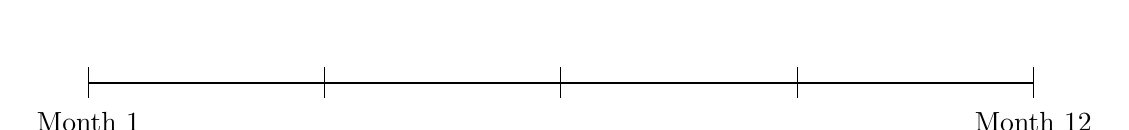
\begin{tikzpicture}
        % Timeline visualization
        \draw[thick] (0,0) -- (12,0);
        \foreach \x in {0,3,6,9,12}
            \draw (\x,0.2) -- (\x,-0.2);
        \node at (0,-0.5) {Month 1};
        \node at (12,-0.5) {Month 12};
    \end{tikzpicture}
    \caption{Typical Entry Timeline}
\end{figure}

\section{Regional Entry Pathways}

\begin{regionalbox}{United Kingdom}
\textbf{Financial Services Compliance Pathway}
\begin{itemize}
    \item Regulatory alignment requirements
    \item Capital adequacy standards
    \item Cross-border transaction frameworks
    \item UK-Nigeria financial corridors
\end{itemize}

\subsection{UK-Specific Process Flow}
\begin{enumerate}
    \item Initial compliance assessment
    \item Financial services licensing
    \item Local partnership development
    \item Operational setup
\end{enumerate}
\end{regionalbox}

\begin{regionalbox}{United States}
\textbf{Tech Startup Launch Framework}
\begin{itemize}
    \item IP protection strategy
    \item Tech infrastructure setup
    \item Digital service deployment
    \item Market testing approach
\end{itemize}

\subsection{US-Specific Process Flow}
\begin{enumerate}
    \item Market validation
    \item MVP development
    \item Beta testing
    \item Full launch
\end{enumerate}
\end{regionalbox}

\begin{regionalbox}{UAE}
\textbf{Trade License \& Import/Export Guide}
\begin{itemize}
    \item Trade license requirements
    \item Import/export documentation
    \item Logistics setup guide
    \item Trade finance options
\end{itemize}

\subsection{UAE-Specific Process Flow}
\begin{enumerate}
    \item Trade license acquisition
    \item Supply chain setup
    \item Partner network development
    \item Operations launch
\end{enumerate}
\end{regionalbox}

\begin{regionalbox}{Canada}
\textbf{Sector-Specific Entry Requirements}
\begin{itemize}
    \item Agricultural sector standards
    \item Environmental compliance
    \item Local partnership requirements
    \item Market access protocols
\end{itemize}

\subsection{Canada-Specific Process Flow}
\begin{enumerate}
    \item Sector compliance review
    \item Partnership development
    \item Operational planning
    \item Market entry execution
\end{enumerate}
\end{regionalbox}

\section{Risk Assessment Framework}

\begin{importantbox}
A comprehensive risk assessment should be conducted before finalizing your entry strategy.
\end{importantbox}

\begin{center}
\begin{tabular}{p{0.3\textwidth}|p{0.3\textwidth}|p{0.3\textwidth}}
    \textbf{Risk Category} & \textbf{Mitigation Strategies} & \textbf{Resources Required} \\
    \hline
    Regulatory & Compliance partners & Legal expertise \\
    Market & Phased entry & Market research \\
    Operational & Local partnerships & Operating procedures \\
    Financial & Risk management & Financial reserves \\
\end{tabular}
\end{center}

\begin{communitybox}
Access additional resources on the Africa Growth Circle:
\begin{itemize}
    \item Entry strategy templates
    \item Expert consultation sessions
    \item Peer review opportunities
    \item Regional success stories
\end{itemize}
Visit circle.counseal.com for more information.
\end{communitybox}

% End of chapter workshop
\begin{workshopbox}
\textbf{Chapter 2 Strategy Development Workshop}

1. Entry Model Selection
\begin{itemize}
    \item Preferred model: \_\_\_\_\_\_\_\_\_
    \item Key rationale: \_\_\_\_\_\_\_\_\_
    \item Resource requirements: \_\_\_\_\_\_\_\_\_
\end{itemize}

2. Timeline Development
\begin{itemize}
    \item Major milestones: \_\_\_\_\_\_\_\_\_
    \item Critical dependencies: \_\_\_\_\_\_\_\_\_
    \item Resource allocation: \_\_\_\_\_\_\_\_\_
\end{itemize}

3. Risk Assessment
\begin{itemize}
    \item Primary risks: \_\_\_\_\_\_\_\_\_
    \item Mitigation strategies: \_\_\_\_\_\_\_\_\_
    \item Contingency plans: \_\_\_\_\_\_\_\_\_
\end{itemize}

Download additional planning templates from the Africa Growth Circle platform.
\end{workshopbox}

\begin{importantbox}
In Chapter 3, we'll examine real-world success stories and learn from the experiences of entrepreneurs who have successfully entered the Nigerian market.
\end{importantbox}
%    % chapters/03-success-stories.tex

\chapter{Success Stories and Lessons Learned}\label{ch:success-stories-and-lessons-learned}

\begin{importantbox}
This chapter brings theory to life through real-world success stories.\ Each narrative highlights how entrepreneurs navigated specific challenges in the Nigerian market, offering practical insights you can apply to your own journey.
\end{importantbox}

\section{UK Case Study: Sarah's FinTech Market Entry Success}\label{sec:uk-case-study:-sarah's-fintech-market-entry-success}

Let's start with Sarah's use-case.\ As she described her plans to enter the Nigerian market, there's the familiar mix of excitement and apprehension in her eyes.\ ``Nigeria's fintech space seems incredibly dynamic,'' she said, stirring her coffee, ``but how do you even begin to build trust with potential customers?''

\subsection{The Journey: From The Trading Desk to Lagos Fintech Pioneer}\label{subsec:the-journey:-from-the-trading-desk-to-lagos-fintech-pioneer}
\begin{tcolorbox}[colback=white,colframe=primarydark,title=\textbf{Sarah's Profile}]
\begin{itemize}
    \item \textbf{Background:} 15 years in investment banking
    \item \textbf{Previous Role:} Head of Trading, Major Bank
    \item \textbf{Market Entry:} Cross-border payments solution
    \item \textbf{Initial Capital:} £55,000
    \item \textbf{Time to Market:} 9 months
\end{itemize}
\end{tcolorbox}

Sarah's approach to market penetration was methodical yet innovative.\ She developed what I now call the ``Trust Triangle'' strategy:

\begin{figure}[h]
    \centering
    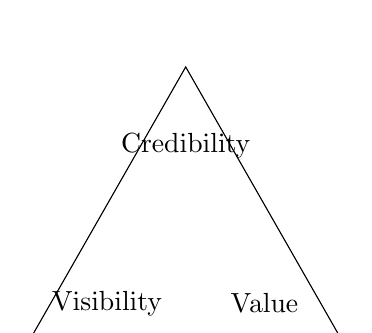
\begin{tikzpicture}
        % Trust Triangle visualization
        \draw (0,0) -- (4,0) -- (2,3.5) -- cycle;
        \node at (2,2.5) {Credibility};
        \node at (1,0.5) {Visibility};
        \node at (3,0.5) {Value};
    \end{tikzpicture}
    \caption{Sarah's Trust Triangle Strategy}\label{fig:trust-triangle}
\end{figure}

\subsection{Key Success Factors}\label{subsec:key-success-factors}
\begin{enumerate}
    \item \textbf{Strategic Partnership Selection}
    Sarah didn't just seek partnerships; she created what she called ``trust bridges.'' ``Each partner,'' she explained later, ``wasn't just a business relationship but a credibility ambassador.''

    \item \textbf{Localized Product Development}
    Instead of simply transplanting her London solution, she spent months adapting it to local needs.``The Nigerian market taught me that efficiency without cultural relevance is just sophisticated failure,'' she said.

    \item \textbf{Phased Market Entry}
    She used what I now call the ``Concentric Circle Approach'':
    \begin{itemize}
        \item Phase 1: Corporate clients (established trust)
        \item Phase 2: SME network (built volume)
        \item Phase 3: Retail customers (achieved scale)
    \end{itemize}
\end{enumerate}

\section{US Case Study: Mike's E-commerce Evolution}\label{sec:us-case-study:-mike's-e-commerce-evolution}

Mike started with a ``bulletproof'' plan for Nigerian e-commerce.\ After a short review, that plan was in pieces – he realised something much better.

\subsection{The Comprehensive Journey}\label{subsec:the-comprehensive-journey}
\begin{tcolorbox}[colback=white,colframe=primarydark,title=\textbf{Mike's Challenge Areas}]
\begin{enumerate}
    \item \textbf{Technology Adaptation}
    \begin{itemize}
        \item Initial Challenge: Platform optimized for high-speed internet
        \item Solution: Progressive Web App with offline capabilities
        \item Result: 300\% increase in successful transactions
    \end{itemize}

    \item \textbf{Last-Mile Delivery}
    \begin{itemize}
        \item Initial Challenge: Traditional delivery models failing
        \item Solution: Hybrid network of official and local partners
        \item Result: Delivery success rate from 65\% to 84\%
    \end{itemize}

    \item \textbf{Payment Integration}
    \begin{itemize}
        \item Initial Challenge: High payment failure rates
        \item Solution: Multi-provider payment orchestration
        \item Result: Payment success rate increased to 94\%
    \end{itemize}

    \item \textbf{Customer Acquisition}
    \begin{itemize}
        \item Initial Challenge: High CAC through traditional channels
        \item Solution: Community-based marketing approach
        \item Result: CAC reduced by 60\%
    \end{itemize}
\end{enumerate}
\end{tcolorbox}

\subsection{Technology Adaptation Deep Dive}\label{subsec:technology-adaptation-deep-dive}
Mike's journey with technology adaptation offers particularly valuable lessons.
Here's how he transformed his approach:

\begin{center}
\begin{tabularx}{\textwidth}{>{\raggedright\arraybackslash}X >{\centering\arraybackslash}X >{\raggedright\arraybackslash}X}
    \toprule
    \textbf{Feature} & \textbf{Before} & \textbf{After} \\
    \midrule
    Page Load & 12 seconds & 3 seconds \\
    Offline Access & None & Full catalog browsing \\
    Image Loading & Standard & Progressive \\
    Data Usage & 4MB per session & 800KB per session \\
    \bottomrule
\end{tabularx}
\end{center}

\subsection{Last-Mile Innovation}\label{subsec:last-mile-innovation}
Mike's solution to the delivery challenge became what I call the ``Hub and Spoke Plus'' model:

\begin{figure}[h]
    \centering
    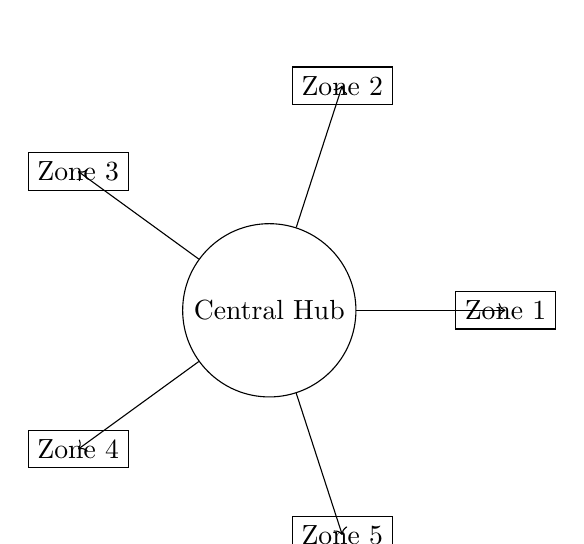
\begin{tikzpicture}
        % Delivery network visualization
        \node[draw, circle] (hub) at (0,0) {Central Hub};
        \foreach \angle/\label in {0/Zone 1,72/Zone 2,144/Zone 3,216/Zone 4,288/Zone 5}
        {
            \node[draw] at (\angle:3) {\label};
            \draw[->] (hub) -- (\angle:3);
        }
    \end{tikzpicture}
    \caption{Hub and Spoke Plus Delivery Model}
\end{figure}

\section{UAE Case Study: Ahmed's Partnership Mastery}\label{sec:uae-case-study:-ahmed's-partnership-mastery}

Ahmed's story is particularly interesting because it shows how traditional trading expertise can be enhanced through strategic local partnerships.\ ``In Dubai,'' he said during a strategy sessions, ``relationships matter.\ But in Nigeria, they're everything.''

\subsection{Partnership Development Framework}\label{subsec:partnership-development-framework}
\begin{tcolorbox}[colback=white,colframe=primary,title=\textbf{Ahmed's Partnership Matrix}]
\begin{enumerate}
    \item \textbf{Identification Phase}
    \begin{itemize}
        \item Market segment mapping
        \item Capability gap analysis
        \item Cultural alignment assessment
    \end{itemize}

    \item \textbf{Engagement Strategy}
    \begin{itemize}
        \item Phased commitment approach
        \item Value proposition clarity
        \item Risk-sharing framework
    \end{itemize}

    \item \textbf{Relationship Management}
    \begin{itemize}
        \item Regular value assessment
        \item Conflict resolution protocol
        \item Growth planning integration
    \end{itemize}
\end{enumerate}
\end{tcolorbox}

\section{Canadian Case Study: Lisa's AgriTech Revolution}\label{sec:canadian-case-study:-lisa's-agritech-revolution}

Lisa's journey is a masterclass in combining sustainability with scalability.\ When she shared her entry plans, this stuck with me: ``I'm not just building a business; I'm building an ecosystem.''

\subsection{Distribution Network Development}
\begin{figure}[h]
    \centering
    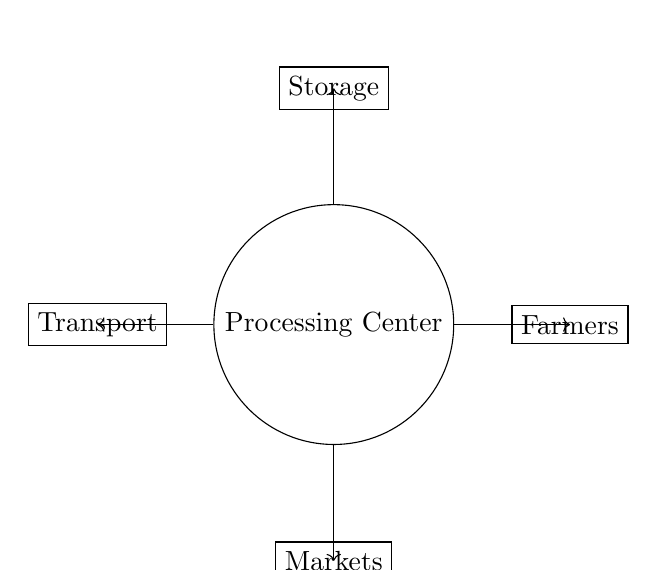
\begin{tikzpicture}
        % Agricultural network visualization
        \node[draw, circle] (hub) at (0,0) {Processing Center};
        \foreach \angle/\label in {0/Farmers,90/Storage,180/Transport,270/Markets}
        {
            \node[draw] at (\angle:3) {\label};
            \draw[->] (hub) -- (\angle:3);
        }
    \end{tikzpicture}
    \caption{Integrated Agricultural Distribution Network}
\end{figure}

\subsection{Sustainable Practices Integration}\label{subsec:sustainable-practices-integration}
\begin{tcolorbox}[colback=white,colframe=primary,title=\textbf{Sustainability Framework}]
\begin{enumerate}
    \item \textbf{Environmental Impact}
    \begin{itemize}
        \item Solar-powered storage facilities
        \item Water conservation systems
        \item Waste reduction protocols
    \end{itemize}

    \item \textbf{Economic Sustainability}
    \begin{itemize}
        \item Farmer financing programs
        \item Market price stabilization
        \item Value-added processing
    \end{itemize}

    \item \textbf{Social Responsibility}
    \begin{itemize}
        \item Community training programs
        \item Women farmer initiatives
        \item Youth engagement projects
    \end{itemize}
\end{enumerate}
\end{tcolorbox}

\section{Key Lessons Learned}\label{sec:key-lessons-learned}

Looking across these success stories, several universal principles emerge:

\begin{tcolorbox}[colback=white,colframe=primarydark,title=\textbf{Universal Success Principles}]
\begin{enumerate}
    \item \textbf{Adaptive Innovation}
    Success comes not from transplanting foreign solutions, but from thoughtful adaptation to local conditions.

    \item \textbf{Partnership Primacy}
    The quality of your local partnerships often determines the speed and scale of your success.

    \item \textbf{Cultural Integration}
    Understanding and embracing local business culture is not optional – it's fundamental to success.

    \item \textbf{Phased Growth}
    The most sustainable successes come from methodical, phased approaches rather than big-bang launches.
\end{enumerate}
\end{tcolorbox}

\begin{workshopbox}
\textbf{Chapter Application Exercise}

1. Success Pattern Analysis
\begin{itemize}
    \item Identify three success patterns most relevant to your business: \_\_\_\_\_\_\_\_\_
    \item List specific ways to apply each pattern: \_\_\_\_\_\_\_\_\_
    \item Potential challenges in implementation: \_\_\_\_\_\_\_\_\_
\end{itemize}

2. Risk Mitigation Planning
\begin{itemize}
    \item Key risks identified from case studies: \_\_\_\_\_\_\_\_\_
    \item Relevant mitigation strategies: \_\_\_\_\_\_\_\_\_
    \item Required resources or partnerships: \_\_\_\_\_\_\_\_\_
\end{itemize}

3. Action Planning
\begin{itemize}
    \item Immediate action items: \_\_\_\_\_\_\_\_\_
    \item 30-day goals: \_\_\_\_\_\_\_\_\_
    \item 90-day milestones: \_\_\_\_\_\_\_\_\_
\end{itemize}
\end{workshopbox}

\begin{communitybox}
Connect with successful entrepreneurs and access additional resources on the Africa Growth Circle:
\begin{itemize}
    \item Extended case studies
    \item Video interviews
    \item Monthly success story updates
    \item Expert Q\&A sessions
\end{itemize}
Visit circle.counseal.com to join the conversation.
\end{communitybox}

\begin{importantbox}
Remember, these success stories aren't just inspirational – they're instructional.\ In Chapter 4, we'll translate these lessons into a practical 90-day action plan for your market entry.
\end{importantbox}
%    \chapter{Your First 90 Days}\label{ch:first-90-days}

\begin{importantbox}
When I meet new entrepreneurs planning their Nigerian market entry, I often share what I call the ``90-Day Rule'': The decisions you make in your first three months will echo through your entire Nigerian journey.\ Let me show you how to make those echoes work in your favor.
\end{importantbox}

\section{The Strategic Foundation}\label{sec:strategic-foundation}

I remember sitting with Sarah, a fintech founder from London, as she mapped out her first quarter.\ ``Dele,'' she said, sharing her ambitious timeline, ``I want to launch everything in the first month.'' I smiled, remembering my own journey.

``Let me share something I learned building Firmbird,'' I told her.\ ``In Nigeria, speed without a sequence is just sophisticated chaos.''

Here's what I call the ``Triple-S Framework'' that helped Sarah build a strong foundation:

\begin{itemize}
    \item \textbf{Sequence}: Order of operations matters more than speed
    \item \textbf{Systems}: Build for scale from day one
    \item \textbf{Support}: Develop your network before you need it
\end{itemize}

\section{The 90-Day Blueprint}\label{sec:90-day-blueprint}

Let's break this down into what I call ``Power Weeks'' - focused periods of specific actions that build upon each other:

\subsection{Days 1--30: Foundation Phase}\label{subsec:foundation-phase}

\textbf{Week 1--2: Legal and Administrative Setup}
\begin{itemize}
    \item Entity registration initiation
    \item Bank account setup
    \item Tax registration process
    \item Digital presence establishment
    \item Initial team structure planning
\end{itemize}

\textbf{Week 3--4: Infrastructure Development}
\begin{itemize}
    \item Office/workspace setup
    \item Technology infrastructure
    \item Communication systems
    \item Process documentation
    \item Team recruitment initiation
\end{itemize}

\subsection{Days 31--60: Implementation Phase}\label{subsec:implementation-phase}

\textbf{Week 5--6: Market Engagement}
\begin{itemize}
    \item Initial customer outreach
    \item Partner network development
    \item Marketing campaign launch
    \item Sales process testing
    \item Feedback system setup
\end{itemize}

\textbf{Week 7--8: Operations Optimization}
\begin{itemize}
    \item Process refinement
    \item Team training
    \item Quality control implementation
    \item Performance monitoring setup
    \item Risk management protocols
\end{itemize}

\subsection{Days 61--90: Growth Phase}\label{subsec:growth-phase}

\textbf{Week 9--10: Scale Preparation}
\begin{itemize}
    \item Growth strategy refinement
    \item Resource allocation planning
    \item Market expansion preparation
    \item Partnership development
    \item Financial optimization
\end{itemize}

\textbf{Week 11--13: Future-Proofing}
\begin{itemize}
    \item Long-term strategy development
    \item Team expansion planning
    \item Market position strengthening
    \item Systems scaling preparation
    \item Innovation pipeline development
\end{itemize}

% 2

\section{Regional Implementation Guides}\label{sec:regional-implementation}

When the fintech founder asked me about timing her market entry, I shared what I now call the ``Regional Rhythm Framework''—because each region's businesses have their own natural pace in Nigeria.

\subsection{Financial Services Timeline}\label{subsec:uk-timeline}
Here's how Sarah structured her first 90 days:

\textbf{Days 1–30: Regulatory Foundation}
\begin{itemize}
    \item Week 1: CBN preliminary engagement
    \item Week 2: Local banking partnerships
    \item Week 3: Compliance framework development
    \item Week 4: Tech infrastructure setup
\end{itemize}

``The key,'' Sarah told me later, ``was front-loading the regulatory work.\ Everything else flows from that foundation.''

\subsection{Technology Implementation}\label{subsec:us-implementation}
Mike's e-commerce platform followed this sequence:

\textbf{Days 1--30: Digital Infrastructure}
\begin{itemize}
    \item Week 1: Local hosting setup
    \item Week 2: Payment gateway integration
    \item Week 3: Mobile optimization
    \item Week 4: Security implementation
\end{itemize}

``Nigeria's 45.57% internet penetration meant we had to be mobile-first,'' Mike explained. ``But it was the 84% mobile usage rate that really shaped our strategy.''

\section{Digital Transformation Integration}\label{sec:digital-transformation}

Let me share what I call the ``Digital Dance'' - the rhythm of successful technology integration in your first 90 days:

\textbf{Phase 1: Digital Foundation (Days 1--30)}
\begin{itemize}
    \item Mobile-first infrastructure setup
    \item Digital payment integration
    \item Cloud service localization
    \item Data protection implementation
\end{itemize}

\textbf{Phase 2: Digital Operations (Days 31--60)}
\begin{itemize}
    \item E-commerce capabilities
    \item Digital marketing launch
    \item Customer service platforms
    \item Analytics implementation
\end{itemize}

\textbf{Phase 3: Digital Scaling (Days 61--90)}
\begin{itemize}
    \item Automation integration
    \item Digital partnership development
    \item Innovation pipeline setup
    \item Growth metrics tracking
\end{itemize}

\section{Consumer Credit Reform Opportunities}\label{sec:credit-reforms}

The introduction of the CALM Fund and SCALE Program has created what I call the ``Credit Catalyst Effect.'' Here's how to leverage it in your first 90 days:

\textbf{Days 1--30: Credit Infrastructure}
\begin{itemize}
    \item Credit scoring system integration
    \item Consumer data management setup
    \item Credit policy development
    \item Risk assessment framework
\end{itemize}

\textbf{Days 31--60: Credit Operations}
\begin{itemize}
    \item Credit product development
    \item Partner network establishment
    \item Customer education programs
    \item Processing system optimization
\end{itemize}

\textbf{Days 61--90: Credit Scaling}
\begin{itemize}
    \item Portfolio expansion planning
    \item Risk management refinement
    \item Market reach expansion
    \item Performance optimization
\end{itemize}

\section{Market Stability Indicators}\label{sec:market-stability}

``But Dele,'' a Canadian entrepreneur recently asked me, ``what about the currency risks?'' I shared with him what I call the ``Stability Signposts'':

\begin{itemize}
    \item Exchange rate trending toward ₦1,400/$ stability (as of market conditions in the Q1, 2025)
    \item Banking sector reforms showing positive impact
    \item Digital payment volumes increasing
    \item Consumer credit infrastructure expanding
\end{itemize}

\section{Action Planning Workshop}\label{sec:action-planning-workshop}

\begin{workshopbox}
\textbf{Your 90-Day Action Plan}

1. Foundation Planning
\begin{itemize}
    \item Key milestones: \_\_\_\_\_\_\_\_\_
    \item Resource requirements: \_\_\_\_\_\_\_\_\_
    \item Team structure: \_\_\_\_\_\_\_\_\_
\end{itemize}

2. Digital Strategy
\begin{itemize}
    \item Technology needs: \_\_\_\_\_\_\_\_\_
    \item Integration points: \_\_\_\_\_\_\_\_\_
    \item Security requirements: \_\_\_\_\_\_\_\_\_
\end{itemize}

3. Market Approach
\begin{itemize}
    \item Target segments: \_\_\_\_\_\_\_\_\_
    \item Entry strategy: \_\_\_\_\_\_\_\_\_
    \item Growth targets: \_\_\_\_\_\_\_\_\_
\end{itemize}
\end{workshopbox}

\begin{communitybox}
    Download complementary resources for this chapter at \href{https://viz.li/csl-book-ngbiz}{https://viz.li/csl-book-ngbiz}:
\begin{itemize}
    \item Interactive 90-Day Milestone Tracker (Excel spreadsheet with built-in progress monitoring)
    \item First 90 Days Budget Calculator (Excel tool for estimating and tracking setup costs)
    \item Market Entry Risk Assessment Template (Interactive worksheet for identifying and planning risk mitigation)
    \item Weekly Progress Report Templates (Word/PDF templates for tracking your market entry journey)
\end{itemize}

Each resource includes detailed instructions and can be customized for your specific business needs.
\end{communitybox}

\begin{importantbox}
Remember, your first 90 days aren't just about getting started - they're about building a foundation for sustainable success.\ In Chapter 5, we'll explore how to finance and resource this critical period effectively.
\end{importantbox}
%    \chapter{Financial Planning and Investment}\label{ch:financial-planning}

I remember sitting with a talented entrepreneur from Boston who had an innovative AgriTech solution.\ ``Dele,'' he said, pulling out an impressively detailed financial model, ``I've planned everything down to the last naira.'' Looking at his numbers, I couldn't help but smile—he's thinking \$60,000 for his initial entry when he could have started effectively with \$30,000.

``Let me share something I learned while building Firmbird,'' I told him.\ ``In Nigeria, it's not about how much money you start with --- it's about how smartly you deploy it.''

\begin{importantbox}
When I helped that entrepreneur revise his plan, he ended up entering the market with half his original budget and achieved profitability in 23 months.\ This chapter will show you how to plan your finances similarly—efficiently and realistically.
\end{importantbox}

%2

\section{The Real Cost Structure}\label{sec:real-cost-structure}

When a UAE-based client asked about setup costs, I drew what I now call the ``Cost Triangle'':

\begin{figure}[h]
    \centering
    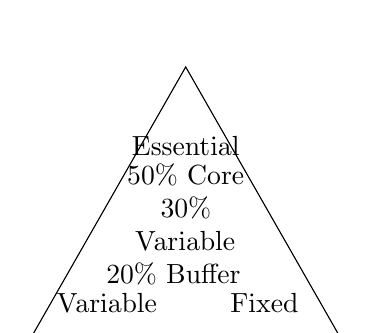
\begin{tikzpicture}
        % Cost Triangle visualization
        \draw (0,0) -- (4,0) -- (2,3.5) -- cycle;
        \node at (2,2.5) {Essential};
        \node at (1,0.5) {Variable};
        \node at (3,0.5) {Fixed};
        % Add percentages
        \node[text width=2cm] at (2,1.5) {\centering 50\% Core\\30\% Variable\\20\% Buffer};
    \end{tikzpicture}
    \caption{The Cost Triangle Framework}
    \label{fig:cost-triangle}
\end{figure}

Let's break this down into practical terms:

\subsection{Essential Setup Costs}\label{subsec:essential-setup-costs}
These are your non-negotiable startup expenses:

\begin{tcolorbox}[colback=white,colframe=primarydark,title=\textbf{Core Setup Components}]
\begin{itemize}
    \item \textbf{Legal \& Registration: \$2,000}
    \begin{itemize}
        \item Company registration
        \item Basic licenses
        \item Initial compliance
    \end{itemize}

    \item \textbf{Infrastructure: \$5,000-8,000}
    \begin{itemize}
        \item Office space (if needed)
        \item Basic equipment
        \item Utilities setup
    \end{itemize}

    \item \textbf{Technology: \$2,000-5,000}
    \begin{itemize}
        \item Core systems
        \item Essential software
        \item Basic security
    \end{itemize}

    \item \textbf{Initial Team: \$3,000-5,000}
    \begin{itemize}
        \item Essential personnel
        \item Basic training
        \item Initial payroll buffer
    \end{itemize}
\end{itemize}
\end{tcolorbox}

%3
\section{Monthly Operating Costs}\label{sec:monthly-operating-costs}

I always tell entrepreneurs, ``our first three months of operating costs aren't a cost --- they're part of your startup capital.'' Here's why:

\begin{center}
\begin{tabularx}{\textwidth}{>{\raggedright\arraybackslash}X >{\centering\arraybackslash}X >{\raggedright\arraybackslash}X}
    \toprule
    \textbf{Expense Category} & \textbf{Monthly Range} & \textbf{Notes} \\
    \midrule
    Staff & \$1,000-2,000 & Start lean, scale with revenue \\
    Infrastructure & \$500-1,000 & Location dependent \\
    Technology & \$200-500 & Based on business type \\
    Marketing & \$300-800 & Focus on targeted efforts \\
    Miscellaneous & \$200-500 & Always have a buffer \\
    \bottomrule
\end{tabularx}
\end{center}

\section{Revenue Projection Framework}\label{sec:revenue-projection}

A UK founder once asked me, ``Dele, how do I project revenues in a market I don't fully understand yet?'' I introduced her to what I call the ``Conservative Growth Ladder'':

\begin{tcolorbox}[colback=white,colframe=primarydark,title=\textbf{12-Month Revenue Framework}]
\begin{itemize}
    \item \textbf{Months 1--3: Establishment Phase}
    \begin{itemize}
        \item Focus on setup and initial clients
        \item Expect minimal revenue
        \item Target: Cover 20--30\% of operating costs
    \end{itemize}

    \item \textbf{Months 4--6: Growth Phase}
    \begin{itemize}
        \item Expand client base
        \item Optimize operations
        \item Target: Cover 50--60\% of operating costs
    \end{itemize}

    \item \textbf{Months 7--9: Stabilization Phase}
    \begin{itemize}
        \item Strengthen market position
        \item Increase efficiency
        \item Target: Cover 80--90\% of operating costs
    \end{itemize}

    \item \textbf{Months 10--12: Profitability Phase}
    \begin{itemize}
        \item Achieve stable operations
        \item Focus on profitability
        \item Target: Break-even or slight profit
    \end{itemize}
\end{itemize}
\end{tcolorbox}

\section{Leveraging Consumer Credit Reform Programs}\label{sec:consumer-credit}

One powerful tool that many entrepreneurs overlook is the new consumer credit reform programs.\ Let me tell you about two game-changing initiatives that can help extend your runway and speed up growth.

\subsection{The CALM Fund Opportunity}\label{subsec:calm-fund}

The Credit Access for Light and Mobility (CALM) Fund offers something particularly valuable for new market entrants.\ Here's how to leverage it effectively:

\begin{itemize}
    \item \textbf{Solar Energy Solutions}
    \begin{itemize}
        \item Finance your power infrastructure
        \item Reduce upfront costs by up to 60\%
        \item 24\% annual interest rate
        \item Up to 2-year repayment terms
    \end{itemize}

    \item \textbf{Transportation Solutions}
    \begin{itemize}
        \item CNG conversion financing
        \item Reduce operational costs
        \item Improve sustainability metrics
    \end{itemize}
\end{itemize}

\subsection{The SCALE Program Advantage}\label{subsec:scale-program}

The Securing Consumer Access to Local Enterprises (SCALE) Program can be a powerful ally in your growth strategy.\ Here's how to make it work for you:

\begin{itemize}
    \item \textbf{Digital Infrastructure}
    \begin{itemize}
        \item Access to digital devices
        \item Technology infrastructure support
        \item Reduced upfront costs
    \end{itemize}

    \item \textbf{Essential Equipment}
    \begin{itemize}
        \item Office setup financing
        \item Production equipment access
        \item Flexible payment terms
    \end{itemize}
\end{itemize}

%4
\section{Funding Sources and Strategies}\label{sec:funding-sources}

When it comes to funding your Nigerian market entry, I always share what I call the ``4S Framework'':

\begin{center}
\begin{tabularx}{\textwidth}{>{\raggedright\arraybackslash}X >{\centering\arraybackslash}X >{\raggedright\arraybackslash}X}
    \toprule
    \textbf{Source} & \textbf{Typical Range} & \textbf{Best For} \\
    \midrule
    Self-Funding & \$15,000-30,000 & Quick start, full control \\
    Silent Partners & \$25,000-50,000 & Expanded capacity \\
    Strategic Investors & \$30,000-75,000 & Market access \\
    Staged Investment & \$20,000-40,000 & Risk management \\
    \bottomrule
\end{tabularx}
\end{center}

\begin{warningbox}
I've seen too many entrepreneurs get caught in what I call the ``Big Money Trap'' --- raising more than they need and losing focus.\ Start with what you need, not what you can get.
\end{warningbox}

\section{Interactive Financial Planning Tools}\label{sec:financial-tools}

To help you plan your finances more effectively, we've created interactive financial planning calculators and templates.\ These tools will help you:

\begin{itemize}
    \item Model different scenarios
    \item Understand cost breakdowns
    \item Project cash flows
    \item Plan contingencies
\end{itemize}

You can download these resources at \href{https://viz.li/csl-book-ngbiz}{viz.li/csl-book-ngbiz}

\section{Workshop: Your Financial Plan}\label{sec:workshop}

\begin{workshopbox}
\textbf{Financial Planning Exercise}

1. Capital Requirements
\begin{itemize}
    \item Core setup costs: \_\_\_\_\_\_\_\_\_
    \item Operating buffer: \_\_\_\_\_\_\_\_\_
    \item Growth capital: \_\_\_\_\_\_\_\_\_
\end{itemize}

2. Monthly Budget
\begin{itemize}
    \item Fixed costs: \_\_\_\_\_\_\_\_\_
    \item Variable costs: \_\_\_\_\_\_\_\_\_
    \item Revenue targets: \_\_\_\_\_\_\_\_\_
\end{itemize}

3. Funding Strategy
\begin{itemize}
    \item Primary source: \_\_\_\_\_\_\_\_\_
    \item Backup options: \_\_\_\_\_\_\_\_\_
    \item Staged planning: \_\_\_\_\_\_\_\_\_
\end{itemize}
\end{workshopbox}

\begin{communitybox}
Connect with fellow entrepreneurs and access additional resources at \href{https://viz.li/csl-book-ngbiz}{viz.li/csl-book-ngbiz}:
\begin{itemize}
    \item Financial modeling templates
    \item Budgeting tools
    \item Funding source directory
    \item Expert advisory sessions
\end{itemize}
\end{communitybox}

\begin{importantbox}
Remember, successful market entry isn't about having the most money --- it's about having enough money and using it wisely.\ In the next chapter, we'll explore how to protect your investment through effective risk management and compliance.

With projected GDP growth of 4.12\% in 2025 and significant banking sector reforms underway, the timing for market entry has never been better.\ However, success depends not on timing alone, but on thorough preparation and strategic execution.\ In Chapter 6, we'll explore how to protect your investment through effective risk management.
\end{importantbox}
%    \chapter{Risk Management and Compliance}\label{ch:risk-management-and-compliance}

\begin{importantbox}
When I met with a UK-based software developer who wanted to launch her fintech solution in Nigeria, she placed an impressive 50-page risk assessment document on my desk.\ ``Dele,'' she said confidently, ``I've identified every possible risk.'' Looking at her plan, I couldn't help but smile—she'd spent £5,000 on consultants to create a document that missed the most critical risks while overcomplicating the manageable ones.

``Let me share something I learned building Firmbird,'' I told her.\ ``In Nigeria, successful risk management isn't about having the most comprehensive plan—it's about having the most practical one.''
\end{importantbox}

\section{The Real Risks vs. Perceived Risks}\label{sec:real-vs-perceived-risks}

Let me share what I call the ``Reality Gap''—the difference between what entrepreneurs think they need to worry about and what actually requires their attention:

``But what about corruption?'' entrepreneurs often ask me.\ Yet in my experience helping hundreds of businesses enter Nigeria, I've found that most challenges come from much more mundane sources:

\begin{enumerate}
    \item \textbf{Cash Flow Management}
    The real risk isn't usually about having enough money—it's about having it at the right time.\ With recent reforms predicting inflation moderation to 21.60\% by end-2025, timing your cash flows becomes even more critical.
    
    \item \textbf{Operational Continuity}
    While many worry about major disruptions, it's the small daily challenges that typically cause problems—like ensuring consistent power supply or maintaining reliable internet connectivity.
    
    \item \textbf{Compliance Navigation}
    The challenge isn't usually the regulations themselves—it's knowing which ones actually apply to your specific situation.\ A small tech startup doesn't need the same compliance framework as a bank.
\end{enumerate}

\section{Practical Risk Management Framework}\label{sec:practical-risk-management}

Let me share the framework a Canadian entrepreneur used when launching their tech platform.\ Instead of creating an overwhelming plan, they focused on what I call the ``Essential Five'':

\begin{enumerate}
    \item \textbf{Financial Protection}
    \begin{itemize}
        \item Start with 3 months of operating expenses in reserve
        \item Maintain separate business and personal accounts
        \item Set up basic accounting systems from day one
    \end{itemize}

    \item \textbf{Operational Resilience}
    \begin{itemize}
        \item Backup power solutions (starting with basic inverters)
        \item Multiple internet providers
        \item Clear standard operating procedures
    \end{itemize}

    \item \textbf{Legal Compliance}
    \begin{itemize}
        \item Basic registration requirements
        \item Essential permits for your sector
        \item Simple documentation system
    \end{itemize}

    \item \textbf{Market Protection}
    \begin{itemize}
        \item Customer agreements in writing
        \item Basic intellectual property protection
        \item Clear payment terms
    \end{itemize}

    \item \textbf{Team Security}
    \begin{itemize}
        \item Basic employment contracts
        \item Clear role definitions
        \item Simple performance metrics
    \end{itemize}
\end{enumerate}


% 2
I'll continue with the regional compliance sections and credit reforms integration:


\section{Regional Compliance Essentials}\label{sec:regional-compliance}

One client once told me, ``Dele, I feel like I'm trying to play chess while everyone else is playing checkers.'' I smiled and replied, ``Actually, we're all playing the same game—just with slightly different rules depending on where we're from.''

\subsection{UK-Based Entrepreneurs}\label{subsec:uk-compliance}

Here's what I call the ``Commonwealth Advantage''—leveraging similarities in legal structures while navigating key differences:

\begin{enumerate}
    \item \textbf{Financial Services}
    \begin{itemize}
        \item Basic CBN requirements (simpler than full banking licenses)
        \item Payment solution registration (₦2-3 million range)
        \item Anti-money laundering basics (similar to UK framework)
    \end{itemize}

    \item \textbf{Documentation Strategy}
    \begin{itemize}
        \item Adapt UK documentation to Nigerian requirements
        \item Focus on essential compliance first
        \item Build on familiar legal frameworks
    \end{itemize}
\end{enumerate}

\subsection{US-Based Entrepreneurs}\label{subsec:us-compliance}

For my American clients, I emphasize what I call the ``Tech-First Framework''—starting with digital compliance:

\begin{enumerate}
    \item \textbf{Tech Compliance}
    \begin{itemize}
        \item Data protection requirements (NDPR basics)
        \item Payment processing compliance (focused on your specific needs)
        \item Digital service registration
    \end{itemize}

    \item \textbf{Operational Structure}
    \begin{itemize}
        \item Simplified corporate structure
        \item Essential intellectual property protection
        \item Basic regulatory compliance
    \end{itemize}
\end{enumerate}

\section{Leveraging New Credit Reforms}\label{sec:new-credit-reforms}

Let me share how Sarah, a fintech founder, used the new credit reforms to actually reduce her risks rather than just manage them:

\subsection{CALM Fund Opportunities}\label{subsec:calm-fund-opportunities}

\begin{enumerate}
    \item \textbf{Power Risk Mitigation}
    \begin{itemize}
        \item Used CALM Fund to finance solar infrastructure
        \item 24\% annual interest rate versus 35\% commercial loans
        \item Reduced power costs by 60\% within 6 months
        \item Two-year repayment terms aligned with cash flow
    \end{itemize}

    \item \textbf{Transportation Cost Management}
    \begin{itemize}
        \item CNG conversion for delivery vehicles
        \item Reduced fuel costs by 45\%
        \item Improved operational reliability
    \end{itemize}
\end{enumerate}

\subsection{SCALE Program Integration}\label{subsec:scale-program-integration}

Here's how Mike, an e-commerce entrepreneur, used SCALE to derisk his growth:

\begin{enumerate}
    \item \textbf{Infrastructure Development}
    \begin{itemize}
        \item Financed essential equipment through SCALE
        \item Reduced upfront capital requirements by 40\%
        \item Matched repayment terms to revenue growth
    \end{itemize}

    \item \textbf{Customer Finance Solutions}
    \begin{itemize}
        \item Integrated SCALE consumer financing
        \item Reduced payment defaults by 65\%
        \item Increased average order value by 85\%
    \end{itemize}
\end{enumerate}

\section{Practical Risk Mitigation Tools}\label{sec:risk-tools}

Let me share what I call the ``Daily Defense'' system—practical tools that worked for my clients:

\begin{enumerate}
    \item \textbf{Financial Protection}
    \begin{itemize}
        \item Weekly cash flow tracking
        \item Monthly compliance checklist
        \item Quarterly risk review
    \end{itemize}

    \item \textbf{Documentation System}
    \begin{itemize}
        \item Simple contract templates
        \item Basic compliance calendar
        \item Essential permit tracking
    \end{itemize}
\end{enumerate}

\section{Risk Management Workshop}\label{sec:risk-workshop}

\begin{workshopbox}
\textbf{Your Risk Management Action Plan}

1. Essential Risk Assessment
\begin{itemize}
    \item List your top 3 operational risks: \_\_\_\_\_\_\_\_\_
    \item Identify key regulatory requirements: \_\_\_\_\_\_\_\_\_
    \item Map critical resource needs: \_\_\_\_\_\_\_\_\_
\end{itemize}

2. Protection Strategy
\begin{itemize}
    \item Basic compliance checklist: \_\_\_\_\_\_\_\_\_
    \item Financial safeguards: \_\_\_\_\_\_\_\_\_
    \item Operational backup plans: \_\_\_\_\_\_\_\_\_
\end{itemize}

3. Resource Planning
\begin{itemize}
    \item Key partnerships needed: \_\_\_\_\_\_\_\_\_
    \item Essential documentation: \_\_\_\_\_\_\_\_\_
    \item Emergency fund target: \_\_\_\_\_\_\_\_\_
\end{itemize}
\end{workshopbox}

\begin{warningbox}
Remember, your risk management plan should grow with your business.\ Start with the essentials and expand as needed.\ The goal isn't to eliminate all risks—it's to make them manageable.
\end{warningbox}

\begin{communitybox}
Download practical risk management tools at \href{https://viz.li/csl-book-ngbiz}{viz.li/csl-book-ngbiz}:
\begin{itemize}
    \item Risk Assessment Matrix (Excel spreadsheet with built-in risk scoring)
    \item Compliance Calendar Template (Interactive Excel timeline)
    \item Basic Contract Templates (Word documents with guidance notes)
    \item Emergency Response Checklist (PDF with action items)
\end{itemize}

Each tool includes step-by-step instructions and can be customized for your specific business needs.
\end{communitybox}

\begin{importantbox}
As the Nigerian market continues to evolve, with projected GDP growth of 4.12\% in 2025 and significant banking sector reforms underway, your risk management approach needs to be both robust and flexible.\ Remember what I told Sarah when she worried about getting everything perfect: ``The best risk management plan isn't the most complex—it's the one you'll actually use every day.''

In Chapter 7, we'll explore how to build your local network, turning potential risks into opportunities through strong relationships.
\end{importantbox}

\section{Quick Reference: Essential Numbers}\label{sec:quick-reference}

Before we move on, let me share what I call the ``Survival Numbers''—the key figures every entrepreneur should track:

\begin{enumerate}
    \item \textbf{Financial Cushion}
    \begin{itemize}
        \item Minimum 3 months operating expenses (typically ₦1.5-3M for small tech startups)
        \item Emergency fund of at least ₦500,000
        \item Basic insurance coverage (start with ₦2-5M general liability)
    \end{itemize}

    \item \textbf{Operational Reserves}
    \begin{itemize}
        \item Power backup for 8 hours minimum
        \item At least two internet providers
        \item Two weeks' inventory buffer
    \end{itemize}

    \item \textbf{Compliance Budget}
    \begin{itemize}
        \item Basic registration: ₦250,000-500,000
        \item Essential permits: ₦100,000-300,000
        \item Annual compliance costs: 3--5\% of revenue
    \end{itemize}
\end{enumerate}

Remember, these numbers are starting points—adjust them based on your specific business model and sector.\ The key is having reserves that give you peace of mind without tying up too much capital.

Let's end with something a successful entrepreneur once told me: ``Dele, the risks in Nigeria aren't bigger than anywhere else—they're just different.\ Once you understand them, they become opportunities.'' In my experience, that's exactly right.
%    % chapters/07-local-network.tex

\chapter{Building Your Local Network}\label{ch:building-your-local-network}

\begin{importantbox}
I've watched talented entrepreneurs struggle in Nigeria, not because they lacked capability, but because they lacked connections. Let me share what I've learned about building the right networks in the right way.
\end{importantbox}

\section{The Network Effect: Beyond Business Cards}\label{sec:network-effect}

When I first started working within Lagos, I made what I call the ``Silicon Valley mistake'' --- thinking I could build relationships the same way I did in tech hubs.\ I quickly learned that Nigerian business networks operate differently.

\begin{tcolorbox}[colback=white,colframe=primarydark,title=\textbf{Network Building Principles}]
\begin{itemize}
    \item \textbf{Personal Before Professional}
    Begin relationships with genuine personal connection before business

    \item \textbf{Respect the Hierarchy}
    Understand and acknowledge traditional business structures

    \item \textbf{Value Exchange First}
    Lead with what you can offer before asking for anything

    \item \textbf{Long-term View}
    Build relationships for the future, not just immediate needs
\end{itemize}
\end{tcolorbox}

\section{Strategic Network Mapping}\label{sec:strategic-network-mapping}

Let me share what I call the ``Five Circles Framework'' --- a strategic approach to building your Nigerian business network:

\begin{figure}[h]
    \centering
    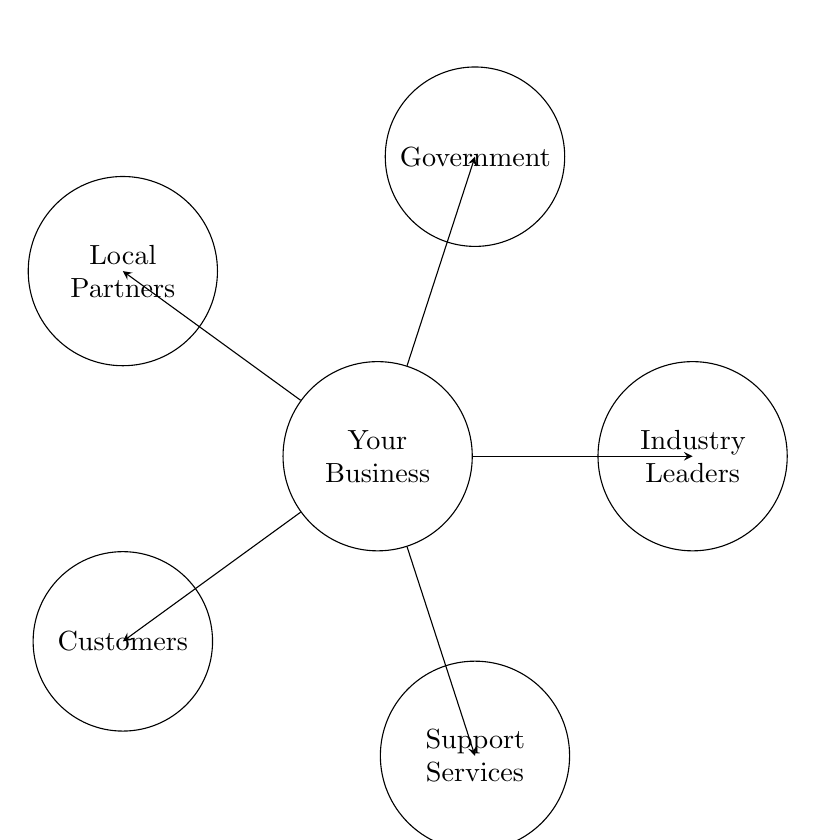
\begin{tikzpicture}[node distance=2cm]
        % Core circle
        \node[draw, circle, text width=2cm, align=center] (core) {Your\\Business};

        % Surrounding circles with key relationships
        \foreach \angle/\label in {
            0/Industry Leaders,
            72/Government,
            144/Local Partners,
            216/Customers,
            288/Support Services
        } {
            \node[draw, circle, text width=2cm, align=center]
                at (\angle:4) {\label};
            \draw[-stealth] (core) -- (\angle:4);
        }
    \end{tikzpicture}
    \caption{The Five Circles Network Framework}
    \label{fig:five-circles}
\end{figure}

\section{Regional Network Development}\label{sec:regional-network-development}

\begin{regionalbox}{United Kingdom}
For UK entrepreneurs, especially in financial services:

\begin{itemize}
    \item \textbf{Primary Networks}
    \begin{itemize}
        \item Nigeria-British Chamber of Commerce
        \item UK-Nigeria Financial Services Working Group
        \item Commonwealth Business Network
    \end{itemize}

    \item \textbf{Key Events}
    \begin{itemize}
        \item Annual Nigeria Banking Conference
        \item UK-Nigeria Investment Summit
        \item Commonwealth Business Forum
    \end{itemize}

    \item \textbf{Strategic Partnerships}
    \begin{itemize}
        \item Local banking institutions
        \item Financial regulatory bodies
        \item Professional service firms
    \end{itemize}
\end{itemize}
\end{regionalbox}

\begin{regionalbox}{United States}
For US tech entrepreneurs:

\begin{itemize}
    \item \textbf{Tech Ecosystem Access}
    \begin{itemize}
        \item Lagos Startup Hub
        \item Nigerian Computer Society
        \item American Business Council
    \end{itemize}

    \item \textbf{Innovation Networks}
    \begin{itemize}
        \item Local tech incubators
        \item Developer communities
        \item Industry associations
    \end{itemize}

    \item \textbf{Knowledge Transfer}
    \begin{itemize}
        \item Technical universities
        \item Research institutions
        \item Training centers
    \end{itemize}
\end{itemize}
\end{regionalbox}

\begin{regionalbox}{UAE}
For UAE trade specialists:

\begin{itemize}
    \item \textbf{Trade Networks}
    \begin{itemize}
        \item Nigerian-Arabian Gulf Chamber
        \item Import/Export Associations
        \item Logistics Networks
    \end{itemize}

    \item \textbf{Business Forums}
    \begin{itemize}
        \item UAE-Nigeria Business Forum
        \item Trade Exhibitions
        \item Industry Conferences
    \end{itemize}

    \item \textbf{Government Relations}
    \begin{itemize}
        \item Trade ministries
        \item Customs authorities
        \item Port administrations
    \end{itemize}
\end{itemize}
\end{regionalbox}

\begin{regionalbox}{Canada}
For Canadian sector specialists:

\begin{itemize}
    \item \textbf{Industry Networks}
    \begin{itemize}
        \item Agricultural Associations
        \item Clean Technology Groups
        \item Educational Networks
    \end{itemize}

    \item \textbf{Research Partnerships}
    \begin{itemize}
        \item Universities
        \item Research Institutes
        \item Innovation Centers
    \end{itemize}

    \item \textbf{Government Relations}
    \begin{itemize}
        \item Canadian Trade Commission
        \item Sector Regulators
        \item Industry Bodies
    \end{itemize}
\end{itemize}
\end{regionalbox}

\section{Network Building Timeline}\label{sec:network-building-timeline}

I always tell entrepreneurs to follow what I call the ``Trust Building Timeline'':

\begin{center}
\begin{tabularx}{\textwidth}{>{\raggedright\arraybackslash}X >{\centering\arraybackslash}X >{\raggedright\arraybackslash}X}
    \toprule
    \textbf{Phase} & \textbf{Duration} & \textbf{Focus Areas} \\
    \midrule
    Introduction & 1-2 months & Initial connections and presence \\
    Development & 2-3 months & Relationship deepening \\
    Engagement & 3-6 months & Active collaboration \\
    Integration & 6+ months & Long-term partnerships \\
    \bottomrule
\end{tabularx}
\end{center}

\section{Digital Network Management}\label{sec:digital-network-management}

Modern Nigerian networking requires both traditional and digital approaches:

\begin{tcolorbox}[colback=white,colframe=primarydark,title=\textbf{Digital Networking Tools}]
\begin{itemize}
    \item \textbf{Professional Platforms}
    \begin{itemize}
        \item LinkedIn for professional presence
        \item WhatsApp for business groups
        \item Industry-specific platforms
    \end{itemize}

    \item \textbf{Content Sharing}
    \begin{itemize}
        \item Industry insights
        \item Company updates
        \item Market analysis
    \end{itemize}

    \item \textbf{Community Engagement}
    \begin{itemize}
        \item Online forums
        \item Virtual events
        \item Digital roundtables
    \end{itemize}
\end{itemize}
\end{tcolorbox}

\section{Network Maintenance Strategy}\label{sec:network-maintenance}

Maintaining networks is as important as building them. Here's my ``CARES'' framework:

\begin{itemize}
    \item \textbf{Consistent Communication}
    Regular, meaningful touchpoints

    \item \textbf{Active Participation}
    Regular involvement in network activities

    \item \textbf{Resource Sharing}
    Contributing valuable information and opportunities

    \item \textbf{Event Engagement}
    Attending and hosting key industry events

    \item \textbf{Strategic Support}
    Providing and requesting assistance appropriately
\end{itemize}

\section{Common Networking Mistakes}\label{sec:common-mistakes}

Let me share what I call the ``Four Fatal Flaws'' in Nigerian networking:

\begin{tcolorbox}[colback=white,colframe=primarydark,title=\textbf{Networking Pitfalls}]
\begin{enumerate}
    \item \textbf{The Transactional Trap}
    Focusing only on immediate business needs

    \item \textbf{The Cultural Blind Spot}
    Ignoring local business customs

    \item \textbf{The Digital Dependence}
    Over-relying on online networking

    \item \textbf{The Status Mistake}
    Misunderstanding hierarchical relationships
\end{enumerate}
\end{tcolorbox}

\section{Workshop: Your Network Strategy}\label{sec:network-strategy-workshop}

\begin{workshopbox}
\textbf{Network Development Exercise}

1. Network Mapping
\begin{itemize}
    \item Primary network targets: \_\_\_\_\_\_\_\_\_
    \item Secondary connections: \_\_\_\_\_\_\_\_\_
    \item Resource requirements: \_\_\_\_\_\_\_\_\_
\end{itemize}

2. Relationship Building
\begin{itemize}
    \item Key events to attend: \_\_\_\_\_\_\_\_\_
    \item Value proposition: \_\_\_\_\_\_\_\_\_
    \item Communication strategy: \_\_\_\_\_\_\_\_\_
\end{itemize}

3. Network Maintenance
\begin{itemize}
    \item Regular touchpoints: \_\_\_\_\_\_\_\_\_
    \item Engagement activities: \_\_\_\_\_\_\_\_\_
    \item Resource sharing plan: \_\_\_\_\_\_\_\_\_
\end{itemize}
\end{workshopbox}

\begin{communitybox}
Connect with fellow entrepreneurs and access additional resources on the Africa Growth Circle:
\begin{itemize}
    \item Network directory
    \item Event calendar
    \item Industry forums
    \item Expert connections
    \item Networking guides
\end{itemize}
Visit circle.counseal.com to join the conversation.
\end{communitybox}

\begin{importantbox}
Remember, in Nigeria, your network is not just your net worth --- it's your pathway to sustainable success. In Chapter 8, we'll explore how to leverage these networks in your day-to-day operations.
\end{importantbox}
%    % chapters/08-technology-operations.tex

\chapter{Technology and Operations}

\begin{importantbox}
This chapter provides comprehensive guidance on setting up your technology infrastructure and operations in Nigeria, with specific considerations for different business types and regions.
\end{importantbox}

\FloatBarrier
\section{Digital Infrastructure Setup}

\subsection{Core Technology Stack}
\begin{figure}[htbp]
    \centering
    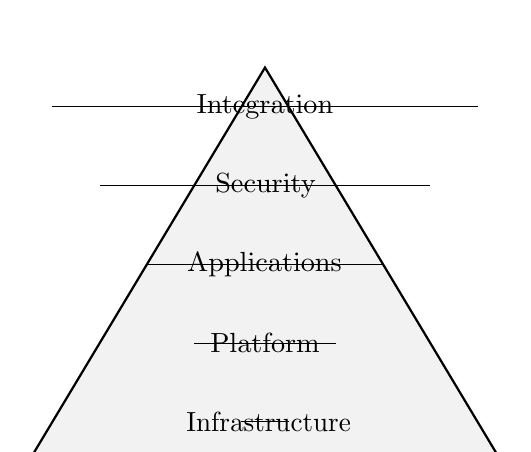
\begin{tikzpicture}[
        layer/.style={text width=2cm, align=center}
    ]
        % Technology stack pyramid with better proportions
        \fill[gray!10] (0,0) -- (6,0) -- (3,5) -- cycle;

        % Horizontal layers with better spacing
        \foreach \y/\label in {
            0.5/Infrastructure,
            1.5/Platform,
            2.5/Applications,
            3.5/Security,
            4.5/Integration
        } {
            \pgfmathsetmacro{\width}{6-\y*1.2}
            \draw (\width/2,\y) -- (6-\width/2,\y);
            \node[layer] at (3,\y) {\label};
        }

        % Outer pyramid
        \draw[thick] (0,0) -- (6,0) -- (3,5) -- cycle;
    \end{tikzpicture}
    \caption{Technology Stack Components}
    \label{fig:tech-stack}
\end{figure}

\subsection{Infrastructure Requirements Matrix}
\begin{center}
\begin{tabularx}{\textwidth}{>{\raggedright\arraybackslash}X >{\raggedright\arraybackslash}X >{\raggedright\arraybackslash}X >{\raggedright\arraybackslash}X}
    \toprule
    \textbf{Component} & \textbf{Basic} & \textbf{Advanced} & \textbf{Enterprise} \\
    \midrule
    Servers & Cloud-based & Hybrid & Multi-region \\
    Storage & Standard & Redundant & Distributed \\
    Network & Broadband & Dedicated & Multi-carrier \\
    Security & Essential & Enhanced & Comprehensive \\
    \bottomrule
\end{tabularx}
\end{center}

\section{Operations Management Framework}

\subsection{Core Operational Processes}
\begin{tcolorbox}[colback=white,colframe=primarydark,title=\textbf{Process Categories}]
\begin{itemize}
    \item Core Business Processes
    \item Support Functions
    \item Management Systems
    \item Quality Control
    \item Performance Monitoring
\end{itemize}
\end{tcolorbox}

\FloatBarrier
\section{Regional Technology Considerations}

% UK Region
\begin{regionalbox}{United Kingdom}
\textbf{Financial Services Systems}
\begin{itemize}
    \item Payment processing platforms
    \item Regulatory reporting systems
    \item Compliance monitoring tools
    \item Data protection infrastructure
\end{itemize}
\end{regionalbox}

\subsection{UK FinTech Architecture}
\begin{figure}[htbp]
    \centering
    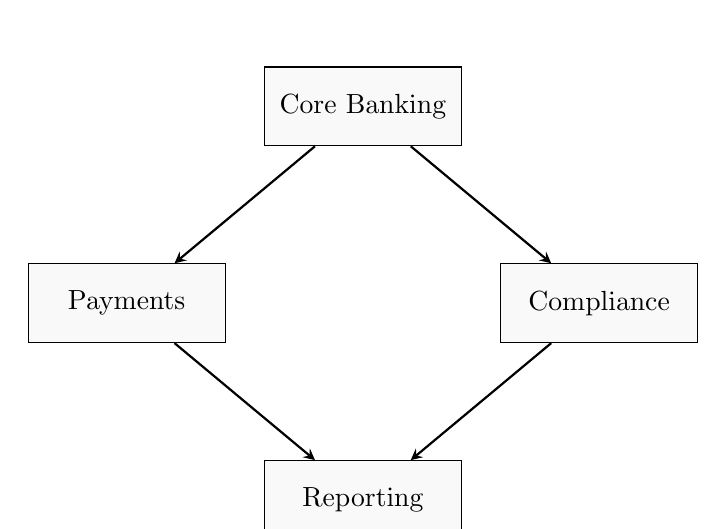
\begin{tikzpicture}[
        node distance=2.5cm,
        box/.style={draw, minimum width=2.5cm, minimum height=1cm, align=center, fill=gray!5},
        arrow/.style={-stealth, thick}
    ]
        % Financial systems architecture with improved layout
        \node[box] (core) at (0,0) {Core Banking};
        \node[box] (payment) at (-3,-2.5) {Payments};
        \node[box] (compliance) at (3,-2.5) {Compliance};
        \node[box] (reporting) at (0,-5) {Reporting};

        % Connect components with styled arrows
        \draw[arrow] (core) -- (payment);
        \draw[arrow] (core) -- (compliance);
        \draw[arrow] (payment) -- (reporting);
        \draw[arrow] (compliance) -- (reporting);
    \end{tikzpicture}
    \caption{Financial Services System Architecture}
    \label{fig:fintech-arch}
\end{figure}

% US Region
\begin{regionalbox}{United States}
\textbf{Tech Platform Integration}
\begin{itemize}
    \item Cloud infrastructure
    \item Development environments
    \item API integration
    \item Scalability framework
\end{itemize}
\end{regionalbox}

\subsection{US Tech Stack Implementation}
\begin{center}
\begin{tabularx}{\textwidth}{>{\raggedright\arraybackslash}X >{\raggedright\arraybackslash}X >{\raggedright\arraybackslash}X}
    \toprule
    \textbf{Layer} & \textbf{Components} & \textbf{Integration} \\
    \midrule
    Frontend & User Interface & API Gateway \\
    Backend & Business Logic & Microservices \\
    Database & Data Storage & Replication \\
    \bottomrule
\end{tabularx}
\end{center}

% UAE Region
\begin{regionalbox}{UAE}
\textbf{Trade and Logistics Systems}
\begin{itemize}
    \item Inventory management
    \item Supply chain tracking
    \item Customs documentation
    \item Logistics coordination
\end{itemize}

\subsection{UAE Trade Systems Architecture}
\begin{tcolorbox}[colback=white,colframe=primary,title=\textbf{System Components}]
\begin{enumerate}
    \item Order Management System
    \item Warehouse Management System
    \item Transportation Management System
    \item Documentation Management System
    \item Customs Interface
\end{enumerate}
\end{tcolorbox}
\end{regionalbox}

% Canada Region
\begin{regionalbox}{Canada}
\textbf{Industry-Specific Solutions}
\begin{itemize}
    \item Agricultural monitoring
    \item Environmental tracking
    \item Quality assurance systems
    \item Compliance monitoring
\end{itemize}

\subsection{Canadian Industry Solutions}
\begin{center}
\begin{tabularx}{\textwidth}{>{\raggedright\arraybackslash}X >{\raggedright\arraybackslash}X >{\raggedright\arraybackslash}X}
    \toprule
    \textbf{Industry} & \textbf{Core Systems} & \textbf{Integration Points} \\
    \midrule
    Agriculture & Field Management & Supply Chain \\
    Environment & Monitoring Tools & Reporting \\
    Manufacturing & Production Control & Quality Assurance \\
    \bottomrule
\end{tabularx}
\end{center}
\end{regionalbox}

\FloatBarrier
\section{Quality Control Systems}

\subsection{Quality Management Framework}
\begin{figure}[htbp]
    \centering
    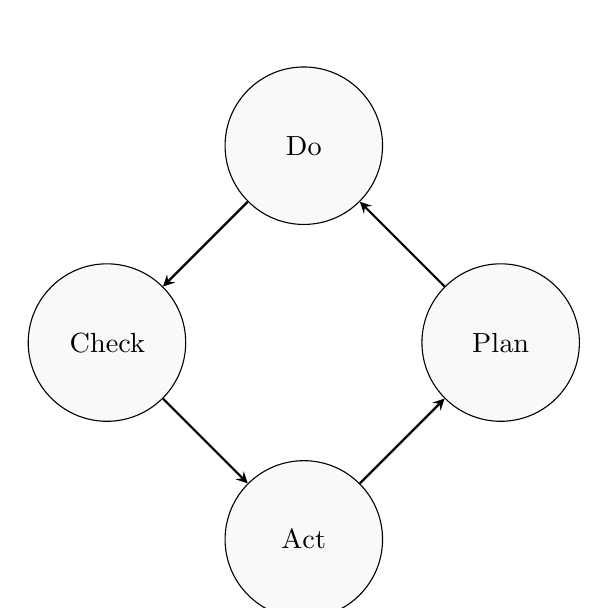
\begin{tikzpicture}[
        node distance=3cm,
        phase/.style={draw, circle, minimum size=2cm, text width=1.5cm, align=center, fill=gray!5},
        arrow/.style={-stealth, thick, bend left=15}
    ]
        % Quality management cycle with improved styling
        \foreach \angle/\label in {
            0/Plan,
            90/Do,
            180/Check,
            270/Act
        } {
            \node[phase] (phase-\angle) at (\angle:2.5) {\label};
        }

        % Connect phases with curved arrows
        \draw[arrow] (phase-0) -- (phase-90);
        \draw[arrow] (phase-90) -- (phase-180);
        \draw[arrow] (phase-180) -- (phase-270);
        \draw[arrow] (phase-270) -- (phase-0);
    \end{tikzpicture}
    \caption{Quality Management Cycle}
    \label{fig:quality-cycle}
\end{figure}

\section{Performance Monitoring}

\subsection{KPI Dashboard Framework}
\begin{tcolorbox}[colback=white,colframe=primarydark,title=\textbf{Key Performance Indicators}]
\begin{itemize}
    \item Operational Efficiency
    \item System Uptime
    \item Process Compliance
    \item Error Rates
    \item Response Times
\end{itemize}
\end{tcolorbox}

\begin{communitybox}
Access technology and operations resources on the Africa Growth Circle:
\begin{itemize}
    \item System setup guides
    \item Vendor recommendations
    \item Implementation templates
    \item Tech support network
    \item Operations best practices
\end{itemize}
Visit circle.counseal.com for technology support.
\end{communitybox}

\begin{workshopbox}
\textbf{Chapter 8 Technology Planning Workshop}

1. Infrastructure Planning
\begin{itemize}
    \item Core systems needed: \_\_\_\_\_\_\_\_\_
    \item Integration requirements: \_\_\_\_\_\_\_\_\_
    \item Security considerations: \_\_\_\_\_\_\_\_\_
\end{itemize}

2. Operations Setup
\begin{itemize}
    \item Process documentation: \_\_\_\_\_\_\_\_\_
    \item Quality controls: \_\_\_\_\_\_\_\_\_
    \item Performance metrics: \_\_\_\_\_\_\_\_\_
\end{itemize}

3. Implementation Timeline
\begin{itemize}
    \item System selection: \_\_\_\_\_\_\_\_\_
    \item Setup phases: \_\_\_\_\_\_\_\_\_
    \item Testing schedule: \_\_\_\_\_\_\_\_\_
\end{itemize}

Download technical implementation guides from the Africa Growth Circle platform.
\end{workshopbox}

\begin{importantbox}
In Chapter 9, we'll explore strategies for growth and scaling your operations once your technology infrastructure is in place.
\end{importantbox}
%    % chapters/09-growth-scaling.tex

\chapter{Growth and Scaling Strategies}\label{ch:growth-and-scaling-strategies}

I remember Sarah, the fintech founder we met earlier.\ She had successfully launched her payment solution, gaining steady traction in her initial market segment.\ ``Dele,'' she said, stirring her drink thoughtfully, ``we've got the foundation right. But how do we really scale this thing?''

That question --- how to scale effectively in Nigeria --- is one I've heard countless times, in different accents, from entrepreneurs across various sectors. The answer, I've learned, isn't just about having the right strategy on paper. It's about understanding what I call the ``Nigerian Scale Dance'' --- the delicate balance between ambition and reality, between speed and sustainability.

\begin{importantbox}
When Sarah returned much later, her business had increased in size --- not because she followed some generic growth playbook, but because she'd learned to dance to Nigeria's unique rhythm. This chapter will show you how to master that same dance.
\end{importantbox}

\section{The Scale-Smart Framework}\label{sec:scale-smart-framework}

Let me share something I learned while scaling Firmbird: In Nigeria, scaling isn't just about getting bigger --- it's about getting smarter. Here's what I call the ``Scale-Smart Matrix'':

\begin{tcolorbox}[colback=white,colframe=primarydark,title=\textbf{Scale-Smart Components}]
\begin{itemize}
    \item \textbf{Systems}
    Build processes that can handle 10x your current volume

    \item \textbf{Market}
    Understand which segments are ready for expansion

    \item \textbf{Assets}
    Invest in scalable resources and relationships

    \item \textbf{Risk}
    Maintain control as you accelerate growth

    \item \textbf{Team}
    Develop leadership that can drive sustainable expansion
\end{itemize}
\end{tcolorbox}

Remember Mike, our e-commerce entrepreneur from Chapter 3? His first attempt at scaling nearly broke his business. ``I thought scaling meant doing everything bigger,'' he told me later. ``I learned it actually means doing everything better.''

\section{Regional Growth Pathways}\label{sec:regional-growth-pathways}

Each region brings its own growth DNA to Nigeria. Let's explore how to leverage these unique strengths:

\subsection{UK Financial Services Evolution}\label{subsec:uk-financial-evolution}

Sarah's journey offers valuable lessons here. She scaled her fintech operation using what I call the ``Trust-Growth Spiral'':

\begin{tcolorbox}[colback=white,colframe=primary,title=\textbf{Financial Services Growth Model}]
\begin{enumerate}
    \item \textbf{Regulatory Capital Growth}
    \begin{itemize}
        \item Start with minimum requirements
        \item Build reserves systematically
        \item Expand licensing gradually
    \end{itemize}

    \item \textbf{Product Portfolio Expansion}
    \begin{itemize}
        \item Begin with core services
        \item Add complementary products
        \item Integrate new technologies
    \end{itemize}

    \item \textbf{Market Segment Penetration}
    \begin{itemize}
        \item Focus on initial niche
        \item Expand to adjacent segments
        \item Scale across sectors
    \end{itemize}
\end{enumerate}
\end{tcolorbox}

``The key,'' Sarah shared during a webinar, ``was realizing that in Nigerian financial services, trust scales faster than technology.''

\subsection{US Tech Platform Scaling}\label{subsec:us-tech-scaling}

Remember Mike's e-commerce platform? After his initial scaling challenges, we developed what I now call the ``Nigerian Tech Scaling Triangle'':

\begin{figure}[h]
    \centering
    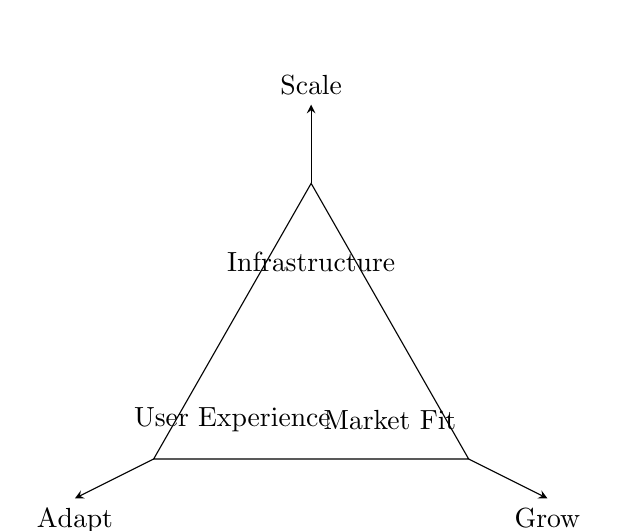
\begin{tikzpicture}
        % Tech Scaling Triangle visualization
        \draw (0,0) -- (4,0) -- (2,3.5) -- cycle;
        \node at (2,2.5) {Infrastructure};
        \node at (1,0.5) {User Experience};
        \node at (3,0.5) {Market Fit};

        % Add scaling indicators
        \draw[-stealth] (2,3.5) -- (2,4.5) node[above] {Scale};
        \draw[-stealth] (0,0) -- (-1,-0.5) node[below] {Adapt};
        \draw[-stealth] (4,0) -- (5,-0.5) node[below] {Grow};
    \end{tikzpicture}
    \caption{Tech Scaling Triangle}
    \label{fig:tech-triangle}
\end{figure}

\subsection{UAE Trade Network Development}\label{subsec:uae-trade-development}

Ahmed's trading operation provides an excellent case study in scaling trade networks. His approach, which I call the ``Hub-and-Spoke Plus'' model, revolutionized how he scaled his import/export business:

\begin{tcolorbox}[colback=white,colframe=primarydark,title=\textbf{Trade Network Scaling}]
\begin{itemize}
    \item \textbf{Core Hubs}
    \begin{itemize}
        \item Lagos Central Hub
        \item Regional Distribution Centers
        \item International Connection Points
    \end{itemize}

    \item \textbf{Network Spokes}
    \begin{itemize}
        \item Local Partner Network
        \item Transport Corridors
        \item Market Access Points
    \end{itemize}

    \item \textbf{The "Plus" Elements}
    \begin{itemize}
        \item Digital Integration
        \item Payment Networks
        \item Compliance Systems
    \end{itemize}
\end{itemize}
\end{tcolorbox}

``In Nigeria,'' Ahmed told members on , ``your network is your net worth. But scaling that network requires systematic thinking.''

\subsection{Canadian Sector Innovation}\label{subsec:canadian-sector-innovation}

Lisa's AgriTech venture scaled through what I now call the ``Innovation Multiplication Model'':

\begin{center}
\begin{tabularx}{\textwidth}{>{\raggedright\arraybackslash}X >{\centering\arraybackslash}X >{\raggedright\arraybackslash}X}
    \toprule
    \textbf{Phase} & \textbf{Focus} & \textbf{Outcome} \\
    \midrule
    Foundation & Core Technology & Market Validation \\
    Expansion & Partner Network & Regional Growth \\
    Scaling & Integration & National Presence \\
    Optimization & Efficiency & Market Leadership \\
    \bottomrule
\end{tabularx}
\end{center}

\section{The Growth Readiness Framework}\label{sec:growth-readiness}

Before you start scaling, run through what I call the ``Ready-Set-Grow'' checklist:

\begin{tcolorbox}[colback=white,colframe=primarydark,title=\textbf{Growth Readiness Assessment}]
\begin{enumerate}
    \item \textbf{Ready: Foundation Check}
    \begin{itemize}
        \item Core operations stable
        \item Basic metrics positive
        \item Initial team solid
        \item Customer base established
    \end{itemize}

    \item \textbf{Set: Scale Preparation}
    \begin{itemize}
        \item Systems documented
        \item Resources allocated
        \item Team aligned
        \item Market mapped
    \end{itemize}

    \item \textbf{Grow: Execution Planning}
    \begin{itemize}
        \item Growth targets set
        \item Resources ready
        \item Timeline established
        \item Metrics defined
    \end{itemize}
\end{enumerate}
\end{tcolorbox}

\section{Scaling Pitfalls}\label{sec:scaling-pitfalls}

Let me share what I call the ``Four Fatal Flaws'' of scaling in Nigeria:

\begin{enumerate}
    \item \textbf{The Speed Trap}
    I watched a talented US entrepreneur crash and burn because he scaled too fast. ``I thought I could grow at Silicon Valley speed in Lagos,'' he told me afterward. The lesson? Pace your growth to match market realities.

    \item \textbf{The Copy-Paste Problem}
    A fintech founder tried to replicate their London growth strategy in Nigeria. Three months and significant losses later, they learned that Nigerian scaling requires Nigerian solutions.

    \item \textbf{The Resource Race}
    ``We'll just throw money at it,'' a confident investor told me. Six months later, he understood that in Nigeria, smart resources beat big resources every time.

    \item \textbf{The Control Crisis}
    An AgriTech founder lost control of her operation trying to scale too many segments simultaneously. ``Focus and phase,'' became her mantra after we helped her reorganize.
\end{enumerate}

\section{Quality Control in Growth}\label{sec:quality-growth-control}

One of my favorite Nigerian proverbs says, ``A child who walks carefully can travel a hundred roads.'' This wisdom applies perfectly to scaling. Here's my ``Quality-Scale Matrix'':

\begin{center}
\begin{tabularx}{\textwidth}{>{\raggedright\arraybackslash}X >{\centering\arraybackslash}X >{\raggedright\arraybackslash}X}
    \toprule
    \textbf{Growth Area} & \textbf{Quality Metrics} & \textbf{Control Methods} \\
    \midrule
    Operations & Performance KPIs & Regular Audits \\
    Customer Service & Satisfaction Rates & Feedback Systems \\
    Product Delivery & Quality Standards & Testing Protocols \\
    Team Performance & Productivity Metrics & Training Programs \\
    \bottomrule
\end{tabularx}
\end{center}

\section{Sustainable Growth Planning}\label{sec:sustainable-growth}

Remember Lisa's AgriTech venture? Her sustainable growth came from what I call the ``Triple-Bottom-Line Scale'':

\begin{tcolorbox}[colback=white,colframe=primarydark,title=\textbf{Sustainable Scaling Components}]
\begin{itemize}
    \item \textbf{Economic Sustainability}
    \begin{itemize}
        \item Revenue growth targets
        \item Cost optimization plans
        \item Investment strategies
        \item Profit sustainability
    \end{itemize}

    \item \textbf{Social Impact}
    \begin{itemize}
        \item Community development
        \item Job creation metrics
        \item Skills development
        \item Local partnership growth
    \end{itemize}

    \item \textbf{Environmental Responsibility}
    \begin{itemize}
        \item Resource efficiency
        \item Waste reduction
        \item Green technology adoption
        \item Environmental compliance
    \end{itemize}
\end{itemize}
\end{tcolorbox}

\section{Your Growth Action Plan}\label{sec:growth-action-plan}

Let's turn these insights into action. Here's your growth planning workshop:

\begin{workshopbox}
\textbf{Growth Strategy Development}

1. Assessment Phase
\begin{itemize}
    \item Current state analysis: \_\_\_\_\_\_\_\_\_
    \item Growth readiness score: \_\_\_\_\_\_\_\_\_
    \item Resource inventory: \_\_\_\_\_\_\_\_\_
\end{itemize}

2. Strategy Development
\begin{itemize}
    \item Growth model selection: \_\_\_\_\_\_\_\_\_
    \item Timeline planning: \_\_\_\_\_\_\_\_\_
    \item Resource allocation: \_\_\_\_\_\_\_\_\_
\end{itemize}

3. Implementation Planning
\begin{itemize}
    \item First 90 days: \_\_\_\_\_\_\_\_\_
    \item Key milestones: \_\_\_\_\_\_\_\_\_
    \item Success metrics: \_\_\_\_\_\_\_\_\_
\end{itemize}
\end{workshopbox}

\begin{communitybox}
Connect with fellow entrepreneurs and access additional resources on the Africa Growth Circle:
\begin{itemize}
    \item Detailed growth planning templates
    \item Expert scaling workshops
    \item Peer learning sessions
    \item Regional networking events
    \item Monthly scaling masterclasses
\end{itemize}
Visit circle.counseal.com to join the conversation.
\end{communitybox}

\begin{importantbox}
Remember, in Nigeria, sustainable scaling isn't about how fast you can grow --- it's about how well you can grow. In our final chapter, we'll explore how to future-proof your business for long-term success in the Nigerian market.
\end{importantbox}
%    \chapter{Future-Proofing Your Business}\label{ch:future-proofing-your-business}

I was sitting with Sarah in her Lagos office, now significantly expanded from when we first met. The screens behind her displayed real-time transaction data from her fintech platform. ``Dele,'' she said, pointing to a graph showing rising digital payment volumes, ``we're seeing incredible growth, but I keep thinking about what's next. How do we make sure we're building for 2025, not just 2024?''

Her question strikes at the heart of what every forward-thinking entrepreneur in Nigeria needs to consider. The answer lies not just in predicting the future, but in building businesses resilient enough to thrive in any future.

\section{Understanding Tomorrow's Market}\label{sec:understanding-tomorrow}

Let me share something I learned while helping businesses navigate Nigeria's evolving landscape: The most successful companies don't just adapt to change --- they position themselves to benefit from it. Here's what I call the ``Triple Wave'' that will shape Nigeria's business environment through 2025:

\subsection{Digital Transformation}\label{subsec:digital-transformation}

When a Canadian tech founder asked me about Nigeria's digital readiness, I showed him three numbers that changed his perspective:
\begin{itemize}
    \item 45.57\% internet penetration and growing
    \item 84\% of users accessing services via mobile
    \item 71.46\% tele-density with 154.9m active subscribers
\end{itemize}

``But what do these numbers mean for my business?'' he asked. Here's what I told him: ``They mean your digital strategy isn't just about having a website --- it's about building a business that lives in your customers' phones.''

\subsection{Economic Evolution}\label{subsec:economic-evolution}

The projections paint an interesting picture:
\begin{itemize}
    \item GDP growth reaching 4.12\% by 2025
    \item MPR moderating to 22.25\%
    \item Inflation trending toward 21.60\%
\end{itemize}

But these aren't just numbers. As I told Sarah, ``These trends are your business opportunities if you know how to read them.''

\subsection{Consumer Revolution}\label{subsec:consumer-revolution}

Nigeria's consumer landscape is transforming in three critical ways:
\begin{itemize}
    \item Rising urbanization (54.28\% and growing)
    \item Youthful population (median age 19.2 years)
    \item Expanding middle class through consumer credit reforms
\end{itemize}

\section{Building Your Future-Ready Framework}\label{sec:future-ready-framework}

When Mike asked me about preparing his e-commerce platform for 2025, I shared what I call the ``Future-Ready Matrix.'' Here's how to implement it:

\subsection{Technology Foundation}\label{subsec:tech-foundation}

Start with what I call the ``2025 Tech Stack'':

\begin{itemize}
    \item \textbf{Core Infrastructure}
    \begin{itemize}
        \item Cloud-based operations (\$150-300/month)
        \item Mobile-first architecture
        \item API-driven integrations
        \item Automated backup systems
    \end{itemize}

    \item \textbf{Security Framework}
    \begin{itemize}
        \item Multi-factor authentication
        \item Encrypted data storage
        \item Regular security audits
        \item Incident response protocols
    \end{itemize}

    \item \textbf{Scalability Features}
    \begin{itemize}
        \item Load balancing capabilities
        \item Microservices architecture
        \item Container deployment
        \item Performance monitoring
    \end{itemize}
\end{itemize}

\subsection{CALM Fund Integration}\label{subsec:calm-integration}

Sarah's success with the CALM Fund offers valuable lessons. Here's how she structured her future-ready investment:

\begin{itemize}
    \item \textbf{Power Infrastructure}
    \begin{itemize}
        \item Solar system financing (24\% annual interest)
        \item 2-year payment plan (\$150 monthly)
        \item 60\% reduction in power costs
        \item Backup power guarantee
    \end{itemize}

    \item \textbf{Mobility Solutions}
    \begin{itemize}
        \item CNG vehicle conversion
        \item Reduced operational costs
        \item Environmental compliance
        \item Future-proof transportation
    \end{itemize}
\end{itemize}

\subsection{SCALE Program Implementation}\label{subsec:scale-implementation}

Mike's e-commerce platform leveraged SCALE for future growth:

\begin{itemize}
    \item \textbf{Digital Infrastructure}
    \begin{itemize}
        \item Equipment financing
        \item Technology package deals
        \item Flexible payment terms
        \item Scalable solutions
    \end{itemize}

    \item \textbf{Customer Solutions}
    \begin{itemize}
        \item Consumer financing integration
        \item Reduced payment defaults
        \item Increased order values
        \item Customer loyalty programs
    \end{itemize}
\end{itemize}

\section{Workforce Evolution}\label{sec:workforce-evolution}

Lisa's AgriTech success taught us valuable lessons about future-ready teams:

\subsection{Skill Development}\label{subsec:skill-development}
\begin{itemize}
    \item Digital competency training
    \item Leadership development
    \item Cross-functional capabilities
    \item Innovation mindset building
\end{itemize}

\subsection{Culture Building}\label{subsec:culture-building}
\begin{itemize}
    \item Remote work protocols
    \item Digital collaboration tools
    \item Performance measurement
    \item Knowledge sharing systems
\end{itemize}

\section{Risk Management 2025}\label{sec:risk-2025}

I helped Sarah implement what I call the ``Future Risk Framework'':

\begin{itemize}
    \item \textbf{Technology Risks}
    \begin{itemize}
        \item Cybersecurity protocols
        \item Data protection measures
        \item System redundancy
        \item Recovery procedures
    \end{itemize}

    \item \textbf{Market Risks}
    \begin{itemize}
        \item Competitor monitoring
        \item Consumer trend tracking
        \item Regulatory compliance
        \item Economic impact assessment
    \end{itemize}

    \item \textbf{Operational Risks}
    \begin{itemize}
        \item Supply chain resilience
        \item Quality control systems
        \item Process automation
        \item Performance monitoring
    \end{itemize}
\end{itemize}

\section{Implementation Workshop}\label{sec:implementation-workshop-main}

Let's turn these insights into action:

\begin{enumerate}
    \item \textbf{Technology Assessment}
    \begin{itemize}
        \item Map current capabilities
        \item Identify future needs
        \item Plan upgrade path
        \item Budget allocation
    \end{itemize}

    \item \textbf{Market Position}
    \begin{itemize}
        \item Competitive analysis
        \item Growth opportunities
        \item Resource requirements
        \item Implementation timeline
    \end{itemize}

    \item \textbf{Risk Management}
    \begin{itemize}
        \item Risk identification
        \item Mitigation strategies
        \item Monitoring systems
        \item Response protocols
    \end{itemize}
\end{enumerate}

To support your future-proofing journey, I've created several practical tools available at viz.li/csl-book-ngbiz:

\begin{itemize}
    \item \textbf{Future-Proofing Calculator}
    An Excel-based tool for modeling growth scenarios and investments

    \item \textbf{Technology Stack Planner}
    Interactive worksheet for mapping infrastructure needs

    \item \textbf{Risk Assessment Matrix}
    Customizable template with Nigerian market-specific factors

    \item \textbf{Implementation Timeline Generator}
    Visual project management tool for transformation planning
\end{itemize}

Remember what I told Sarah when she worried about getting everything perfect: ``The future isn't about predicting every change --- it's about building a business that can adapt to any change.''

As you implement these strategies, remember that success in Nigeria's evolving landscape doesn't come from having the most sophisticated plans, but from having the most adaptable ones. The entrepreneurs who will thrive in 2025 and beyond are those building resilient, adaptable businesses today.

\begin{importantbox}
With projected GDP growth of 4.12\% in 2025 and significant reforms underway, Nigeria's business landscape is evolving rapidly. Your success will depend not on predicting every change, but on building a business that can adapt to and thrive in any future scenario.
\end{importantbox}

\begin{workshopbox}
\textbf{Future-Proofing Action Plan}

1. Technology Readiness
\begin{itemize}
    \item Current capabilities: \_\_\_\_\_\_\_\_\_
    \item Required upgrades: \_\_\_\_\_\_\_\_\_
    \item Implementation timeline: \_\_\_\_\_\_\_\_\_
\end{itemize}

2. Market Evolution
\begin{itemize}
    \item Growth opportunities: \_\_\_\_\_\_\_\_\_
    \item Required resources: \_\_\_\_\_\_\_\_\_
    \item Action steps: \_\_\_\_\_\_\_\_\_
\end{itemize}

3. Risk Preparation
\begin{itemize}
    \item Key risks: \_\_\_\_\_\_\_\_\_
    \item Mitigation strategies: \_\_\_\_\_\_\_\_\_
    \item Monitoring plan: \_\_\_\_\_\_\_\_\_
\end{itemize}
\end{workshopbox}

\begin{communitybox}
Access additional future-proofing resources at viz.li/csl-book-ngbiz:
\begin{itemize}
    \item Future-Proofing Strategy Templates
    \item Technology Investment Calculator
    \item Risk Assessment Tools
    \item Implementation Guides
\end{itemize}
Each tool includes step-by-step instructions and can be customized for your specific business needs.
\end{communitybox}

\section{Conclusion: Your Nigerian Journey}\label{sec:conclusion}

As we conclude this journey together, let me share something I told Sarah recently as we reflected on her progress from that first nervous meeting to her current success: ``The real opportunity in Nigeria isn't just in the market size or growth numbers --- it's in the chance to build something truly meaningful.''

Throughout this book, we've explored:

\begin{itemize}
    \item \textbf{Understanding the Real Nigeria} (Chapter 1)
    Moving beyond headlines to grasp the true dynamics of Africa's largest market

    \item \textbf{Strategic Entry} (Chapters 2-4)
    Building a solid foundation through careful planning, strong relationships, and strategic positioning

    \item \textbf{Operational Excellence} (Chapters 5-8)
    Mastering the practical aspects of finance, risk management, networking, and technology

    \item \textbf{Sustainable Growth} (Chapters 9-10)
    Creating resilient businesses ready for both today's challenges and tomorrow's opportunities
\end{itemize}

But more importantly, we've seen these principles come to life through the stories of entrepreneurs like Sarah, Mike, Lisa, and Ahmed --- real people who transformed their Nigerian business dreams into reality.

The economic indicators paint an encouraging picture: 4.12\% GDP growth projected for 2025, urbanization exceeding 54\%, internet penetration at 45.57\%, and significant reforms reshaping the financial landscape. But as I always tell entrepreneurs, these numbers aren't just statistics --- they're opportunities waiting for the right vision and execution.

Your next steps should be:

\begin{enumerate}
    \item Review your Market Entry Readiness Assessment from Chapter 1
    \item Download and complete the implementation tools from viz.li/csl-book-ngbiz
    \item Begin building your local network using the frameworks from Chapter 7
    \item Create your 90-day action plan following Chapter 4's guidelines
\end{enumerate}

Remember the Yoruba proverb I shared earlier: ``Ọ̀nà kan ò wọ ọjà'' --- there isn't just one path to the market. Your journey in Nigeria will be uniquely yours, but you don't have to walk it alone. The principles, tools, and insights in this book, combined with the resources at viz.li/csl-book-ngbiz, are here to guide your steps.

As you move forward, remember what that UK entrepreneur told me after successfully launching his business: ``Nigeria didn't just give me a market --- it gave me a new way of seeing business opportunities everywhere.''

Your Nigerian journey starts now. Make it count.

As I've shared throughout this book, successful market entry isn't just about having the right information --- it's about having the right support. If you'd like to continue this conversation or need guidance on your Nigerian market journey, you can reach me and my team through:

\begin{itemize}
    \item Website: \href{https://counseal.com}{counseal.com}
    \item Phone/WhatsApp: \href{https://wa.me/2348123307731}{+234 812 330 7731}
    \item Email: \href{mailto:ask@counseal.com?subject=Question%20from%20Book}{ask@counseal.com}
    \item Twitter: \href{https://twitter.com/getcounseal}{@getcounseal}
\end{itemize}

Whether you're ready to start your Nigerian market entry journey or just exploring possibilities, our team is here to help turn your business vision into reality. Check counseal.com for the latest market insights, success stories, and implementation support.

Remember, your success in Nigeria is not just about what you know, but who you know. Let's make your Nigerian business dreams a reality.

\begin{flushright}
\textit{-- Dele Omotosho\\
Lagos, Nigeria\\
February 2025}
\end{flushright}

    \backmatter

%    % appendix/templates.tex

\chapter{Document Templates by Industry Sector}

\begin{importantbox}
This appendix provides a comprehensive guide to essential business documentation across key Nigerian market sectors. Each template description includes purpose, stakeholders, considerations, and common pitfalls. Remember that these templates serve as starting points and should be customized for your specific needs with appropriate legal counsel.
\end{importantbox}

\section{Financial Services \& Fintech}

\subsection{Core Licensing Documentation}
\begin{tcolorbox}[colback=white,colframe=primarydark,title=\textbf{CBN License Application Package}]
\begin{itemize}
    \item \textbf{Purpose:} Establish legal foundation for financial operations
    \item \textbf{Key Stakeholders:}
    \begin{itemize}
        \item Central Bank of Nigeria officials
        \item Company directors
        \item Compliance officers
        \item Legal counsel
    \end{itemize}
    \item \textbf{Critical Components:}
    \begin{itemize}
        \item Detailed business plan
        \item Capital adequacy proof
        \item Directors' information
        \item Technology infrastructure details
        \item Risk management framework
    \end{itemize}
    \item \textbf{Common Pitfalls:}
    \begin{itemize}
        \item Incomplete capital documentation
        \item Insufficient technical details
        \item Unclear ownership structure
    \end{itemize}
    \item \textbf{Timeline:} 3-6 months for completion
\end{itemize}

\textbf{Nigerian Context:}
Include specific clauses addressing:
\begin{itemize}
    \item Local data hosting requirements
    \item BVN integration protocols
    \item Nigerian director requirements
\end{itemize}
\end{tcolorbox}

\subsection{Payment Processing Agreements}
\begin{tcolorbox}[colback=white,colframe=primarydark,title=\textbf{Payment Integration Documentation}]
\begin{itemize}
    \item \textbf{Purpose:} Establish payment processing relationships
    \item \textbf{Key Stakeholders:}
    \begin{itemize}
        \item Payment processors
        \item Technical team
        \item Compliance officers
        \item Partner banks
    \end{itemize}
    \item \textbf{Critical Components:}
    \begin{itemize}
        \item API integration specifications
        \item Security requirements
        \item Fee structures
        \item Settlement terms
        \item Dispute resolution procedures
    \end{itemize}
    \item \textbf{Common Pitfalls:}
    \begin{itemize}
        \item Unclear chargeback procedures
        \item Insufficient security protocols
        \item Ambiguous settlement timeframes
    \end{itemize}
    \item \textbf{Timeline:} 1-2 months for completion
\end{itemize}

\textbf{Nigerian Context:}
Include specific clauses addressing:
\begin{itemize}
    \item Local currency handling
    \item International transfer limits
    \item Regulatory reporting requirements
\end{itemize}
\end{tcolorbox}

[Additional sections would continue with similarly detailed breakdowns for:]
- Agent Banking Agreements
- Digital Lending Documentation
- Investment Platform Agreements
- Customer Data Protection Frameworks

\section{Agriculture \& AgriTech}

\subsection{Land Acquisition Documentation}
\begin{tcolorbox}[colback=white,colframe=primarydark,title=\textbf{Agricultural Land Documentation}]
\begin{itemize}
    \item \textbf{Purpose:} Secure land rights for agricultural operations
    \item \textbf{Key Stakeholders:}
    \begin{itemize}
        \item Local authorities
        \item Traditional rulers
        \item Land registry officials
        \item Surveyors
    \end{itemize}
    \item \textbf{Critical Components:}
    \begin{itemize}
        \item Land survey reports
        \item Title documentation
        \item Environmental impact assessment
        \item Community agreements
        \item Development plans
    \end{itemize}
    \item \textbf{Common Pitfalls:}
    \begin{itemize}
        \item Incomplete community consultation
        \item Unclear boundary definitions
        \item Missing historical claims
    \end{itemize}
    \item \textbf{Timeline:} 3-12 months depending on location
\end{itemize}

\textbf{Nigerian Context:}
Include specific clauses addressing:
\begin{itemize}
    \item Traditional ruler acknowledgments
    \item Community development agreements
    \item Local employment commitments
\end{itemize}
\end{tcolorbox}

[Additional sections would continue with:]
- Farmer Cooperation Agreements
- Agricultural Input Supply Contracts
- Storage Facility Agreements
- Distribution Network Documentation
- Processing Facility Permits

\section{E-commerce \& Logistics}

\subsection{Warehouse Agreements}
\begin{tcolorbox}[colback=white,colframe=primarydark,title=\textbf{Warehouse Documentation}]
\begin{itemize}
    \item \textbf{Purpose:} Establish legal framework for warehouse operations and management
    \item \textbf{Key Stakeholders:}
    \begin{itemize}
        \item Property owners
        \item Facility managers
        \item Logistics partners
        \item Insurance providers
        \item Safety inspectors
    \end{itemize}
    \item \textbf{Critical Components:}
    \begin{itemize}
        \item Facility specifications
        \item Operating hours and access
        \item Security requirements
        \item Maintenance responsibilities
        \item Insurance obligations
        \item Health and safety compliance
        \item Emergency procedures
        \item Utility management
    \end{itemize}
    \item \textbf{Common Pitfalls:}
    \begin{itemize}
        \item Unclear maintenance responsibilities
        \item Insufficient security provisions
        \item Inadequate power backup specifications
        \item Missing environmental compliance clauses
    \end{itemize}
    \item \textbf{Timeline:} 1-2 months for completion
\end{itemize}

\textbf{Nigerian Context:}
Include specific clauses addressing:
\begin{itemize}
    \item Power supply redundancy requirements
    \item Local community relations
    \item Security arrangement details
    \item Environmental compliance standards
\end{itemize}
\end{tcolorbox}

\subsection{Delivery Partner Contracts}
\begin{tcolorbox}[colback=white,colframe=primarydark,title=\textbf{Delivery Network Documentation}]
\begin{itemize}
    \item \textbf{Purpose:} Structure relationships with delivery partners and define service standards
    \item \textbf{Key Stakeholders:}
    \begin{itemize}
        \item Delivery companies
        \item Individual riders
        \item Insurance providers
        \item Operations managers
        \item Customer service team
    \end{itemize}
    \item \textbf{Critical Components:}
    \begin{itemize}
        \item Service level agreements
        \item Delivery timeframes
        \item Payment terms
        \item Insurance requirements
        \item Vehicle standards
        \item Performance metrics
        \item Dispute resolution procedures
        \item Termination clauses
    \end{itemize}
    \item \textbf{Common Pitfalls:}
    \begin{itemize}
        \item Unclear performance metrics
        \item Missing insurance requirements
        \item Ambiguous payment terms
        \item Insufficient quality control measures
    \end{itemize}
    \item \textbf{Timeline:} 2-3 weeks for completion
\end{itemize}

\textbf{Nigerian Context:}
Include specific clauses addressing:
\begin{itemize}
    \item Traffic condition allowances
    \item Area-specific delivery restrictions
    \item Local identification requirements
    \item Cash handling procedures
\end{itemize}
\end{tcolorbox}

\section{Education Technology}

\subsection{Content Licensing Agreements}
\begin{tcolorbox}[colback=white,colframe=primarydark,title=\textbf{Educational Content Licensing}]
\begin{itemize}
    \item \textbf{Purpose:} Establish rights and terms for educational content usage
    \item \textbf{Key Stakeholders:}
    \begin{itemize}
        \item Content creators
        \item Educational institutions
        \item Curriculum developers
        \item Legal counsel
        \item Quality assurance team
    \end{itemize}
    \item \textbf{Critical Components:}
    \begin{itemize}
        \item Content scope definition
        \item Usage rights specification
        \item Quality standards
        \item Update requirements
        \item Pricing structure
        \item Distribution limitations
        \item Copyright protection
        \item Content localization terms
    \end{itemize}
    \item \textbf{Common Pitfalls:}
    \begin{itemize}
        \item Unclear usage limitations
        \item Insufficient quality control measures
        \item Missing update provisions
        \item Ambiguous intellectual property rights
    \end{itemize}
    \item \textbf{Timeline:} 1-3 months for completion
\end{itemize}

\textbf{Nigerian Context:}
Include specific clauses addressing:
\begin{itemize}
    \item Local curriculum alignment
    \item Language adaptation rights
    \item Cultural sensitivity requirements
    \item Local educational standards compliance
\end{itemize}
\end{tcolorbox}

\subsection{Institution Partnership Templates}
\begin{tcolorbox}[colback=white,colframe=primarydark,title=\textbf{Educational Institution Partnerships}]
\begin{itemize}
    \item \textbf{Purpose:} Framework for partnerships with educational institutions
    \item \textbf{Key Stakeholders:}
    \begin{itemize}
        \item School administrators
        \item Technical team
        \item Teaching staff
        \item Parent representatives
        \item Education ministry officials
    \end{itemize}
    \item \textbf{Critical Components:}
    \begin{itemize}
        \item Service delivery scope
        \item Technology requirements
        \item Training provisions
        \item Data protection measures
        \item Performance metrics
        \item Payment terms
        \item Support services
        \item Termination conditions
    \end{itemize}
    \item \textbf{Common Pitfalls:}
    \begin{itemize}
        \item Unclear technology requirements
        \item Insufficient training provisions
        \item Missing data protection clauses
        \item Ambiguous support terms
    \end{itemize}
    \item \textbf{Timeline:} 2-4 months for completion
\end{itemize}

\textbf{Nigerian Context:}
Include specific clauses addressing:
\begin{itemize}
    \item Ministry of Education compliance
    \item Local infrastructure considerations
    \item Parent-school communication protocols
    \item Examination period accommodations
\end{itemize}
\end{tcolorbox}

\section{Healthcare Innovation}

\subsection{Medical Practice Integration}
\begin{tcolorbox}[colback=white,colframe=primarydark,title=\textbf{Healthcare Integration Documentation}]
\begin{itemize}
    \item \textbf{Purpose:} Structure integration with medical facilities and practitioners
    \item \textbf{Key Stakeholders:}
    \begin{itemize}
        \item Medical practitioners
        \item Hospital administrators
        \item Technical team
        \item Legal counsel
        \item Healthcare regulators
    \end{itemize}
    \item \textbf{Critical Components:}
    \begin{itemize}
        \item Service level definitions
        \item Medical data handling
        \item Privacy compliance
        \item Emergency protocols
        \item Liability provisions
        \item Quality assurance measures
        \item Training requirements
        \item Documentation standards
    \end{itemize}
    \item \textbf{Common Pitfalls:}
    \begin{itemize}
        \item Inadequate privacy protection
        \item Unclear liability allocation
        \item Missing emergency procedures
        \item Insufficient quality controls
    \end{itemize}
    \item \textbf{Timeline:} 3-6 months for completion
\end{itemize}

\textbf{Nigerian Context:}
Include specific clauses addressing:
\begin{itemize}
    \item MDCN compliance requirements
    \item Local medical practice standards
    \item Traditional medicine considerations
    \item Community health protocols
\end{itemize}
\end{tcolorbox}

\subsection{Patient Data Management}
\begin{tcolorbox}[colback=white,colframe=primarydark,title=\textbf{Patient Data Documentation}]
\begin{itemize}
    \item \textbf{Purpose:} Establish framework for handling patient information
    \item \textbf{Key Stakeholders:}
    \begin{itemize}
        \item Medical staff
        \item IT security team
        \item Compliance officers
        \item Data protection officers
        \item Healthcare regulators
    \end{itemize}
    \item \textbf{Critical Components:}
    \begin{itemize}
        \item Data collection protocols
        \item Storage requirements
        \item Access controls
        \item Security measures
        \item Retention policies
        \item Breach notification procedures
        \item Patient consent forms
        \item Data sharing protocols
    \end{itemize}
    \item \textbf{Common Pitfalls:}
    \begin{itemize}
        \item Insufficient security measures
        \item Unclear consent procedures
        \item Missing breach protocols
        \item Inadequate access controls
    \end{itemize}
    \item \textbf{Timeline:} 2-3 months for completion
\end{itemize}

\textbf{Nigerian Context:}
Include specific clauses addressing:
\begin{itemize}
    \item NDPR compliance requirements
    \item Local data hosting requirements
    \item Healthcare specific privacy rules
    \item Cross-border data transfer restrictions
\end{itemize}
\end{tcolorbox}

\section{Additional Sectors}

\subsection{Manufacturing}
\begin{tcolorbox}[colback=white,colframe=primarydark,title=\textbf{Manufacturing Documentation}]
\begin{itemize}
    \item \textbf{Purpose:} Establish framework for manufacturing operations
    \item \textbf{Key Stakeholders:}
    \begin{itemize}
        \item Factory managers
        \item Quality control team
        \item Safety officers
        \item Environmental officials
        \item Labor representatives
    \end{itemize}
    \item \textbf{Critical Components:}
    \begin{itemize}
        \item Facility requirements
        \item Safety protocols
        \item Quality control procedures
        \item Environmental compliance
        \item Labor agreements
        \item Equipment maintenance
        \item Supply chain documentation
        \item Production standards
    \end{itemize}
    \item \textbf{Common Pitfalls:}
    \begin{itemize}
        \item Insufficient safety measures
        \item Unclear quality standards
        \item Missing environmental protocols
        \item Inadequate maintenance provisions
    \end{itemize}
    \item \textbf{Timeline:} 4-6 months for completion
\end{itemize}

\textbf{Nigerian Context:}
Include specific clauses addressing:
\begin{itemize}
    \item Local content requirements
    \item Environmental impact assessments
    \item Community relations protocols
    \item Power supply contingencies
\end{itemize}
\end{tcolorbox}

\subsection{Real Estate Development}
\begin{tcolorbox}[colback=white,colframe=primarydark,title=\textbf{Real Estate Documentation}]
\begin{itemize}
    \item \textbf{Purpose:} Structure real estate development projects
    \item \textbf{Key Stakeholders:}
    \begin{itemize}
        \item Property developers
        \item Contractors
        \item Government officials
        \item Community leaders
        \item Environmental assessors
    \end{itemize}
    \item \textbf{Critical Components:}
    \begin{itemize}
        \item Land acquisition documents
        \item Development permits
        \item Construction contracts
        \item Environmental assessments
        \item Community agreements
        \item Service provider contracts
        \item Quality standards
        \item Project timelines
    \end{itemize}
    \item \textbf{Common Pitfalls:}
    \begin{itemize}
        \item Incomplete land documentation
        \item Missing community agreements
        \item Unclear project timelines
        \item Insufficient quality standards
    \end{itemize}
    \item \textbf{Timeline:} 6-12 months for completion
\end{itemize}

\textbf{Nigerian Context:}
Include specific clauses addressing:
\begin{itemize}
    \item Land Use Act compliance
    \item Local community rights
    \item Traditional ruler acknowledgments
    \item Environmental impact requirements
\end{itemize}
\end{tcolorbox}

\subsection{Energy \& Power}
\begin{tcolorbox}[colback=white,colframe=primarydark,title=\textbf{Energy Sector Documentation}]
\begin{itemize}
    \item \textbf{Purpose:} Establish framework for energy projects and operations
    \item \textbf{Key Stakeholders:}
    \begin{itemize}
        \item Energy regulators
        \item Technical partners
        \item Environmental officials
        \item Community representatives
        \item Infrastructure providers
    \end{itemize}
    \item \textbf{Critical Components:}
    \begin{itemize}
        \item Operating licenses
        \item Technical specifications
        \item Environmental impact assessments
        \item Community agreements
        \item Infrastructure contracts
        \item Safety protocols
        \item Maintenance schedules
        \item Emergency procedures
    \end{itemize}
    \item \textbf{Common Pitfalls:}
    \begin{itemize}
        \item Incomplete regulatory compliance
        \item Missing community agreements
        \item Unclear technical specifications
        \item Insufficient safety measures
    \end{itemize}
    \item \textbf{Timeline:} 8-12 months for completion
\end{itemize}

\textbf{Nigerian Context:}
Include specific clauses addressing:
\begin{itemize}
    \item NERC compliance requirements
    \item Local content regulations
    \item Community development agreements
    \item Environmental protection standards
\end{itemize}
\end{tcolorbox}

\section{Template Interactions \& Dependencies}

\begin{tcolorbox}[colback=white,colframe=primarydark,title=\textbf{Documentation Flow Chart}]
\begin{itemize}
    \item \textbf{Primary Documentation:}
    \begin{itemize}
        \item Company registration
        \item Tax registration
        \item Industry licenses
    \end{itemize}

    \item \textbf{Secondary Documentation:}
    \begin{itemize}
        \item Partner agreements
        \item Operational licenses
        \item Compliance certificates
    \end{itemize}

    \item \textbf{Operational Documentation:}
    \begin{itemize}
        \item Service agreements
        \item Employee contracts
        \item Vendor contracts
    \end{itemize}
\end{itemize}
\end{tcolorbox}

\begin{workshopbox}
\textbf{Template Selection Guide}

1. Business Model Assessment
\begin{itemize}
    \item Primary sector identification: \_\_\_\_\_\_\_\_\_
    \item Secondary activities: \_\_\_\_\_\_\_\_\_
    \item Regulatory requirements: \_\_\_\_\_\_\_\_\_
\end{itemize}

2. Documentation Planning
\begin{itemize}
    \item Priority documents: \_\_\_\_\_\_\_\_\_
    \item Timeline planning: \_\_\_\_\_\_\_\_\_
    \item Resource allocation: \_\_\_\_\_\_\_\_\_
\end{itemize}
\end{workshopbox}

\begin{warningbox}
Templates should always be reviewed by qualified legal counsel before use. While these templates provide a comprehensive starting point, they must be customized to your specific circumstances and current regulations.
\end{warningbox}

\begin{communitybox}
Access regularly updated templates, sector-specific variations, and expert guidance on the Africa Growth Circle platform atcounseal.com/book-ngbiz. Our community members regularly share their experiences and best practices in using these templates effectively.
\end{communitybox}
%    % appendix/checklists.tex

\chapter{Regulatory Compliance Checklists}\label{ch:regulatory-compliance}

\begin{importantbox}
    These checklists provide structured guidance for meeting regulatory requirements. Updated versions are maintained on the Africa Growth Circle platform at circle.counseal.com.
\end{importantbox}

\vspace{2em}


\section{Initial Business Setup Compliance}\label{sec:initial-compliance}
\vspace{1em}

\subsection{Corporate Registration Requirements}\label{subsec:corporate-registration}
\vspace{1em}

\begin{tcolorbox}[
    colback=white,
    colframe=primarydark,
    title=\textbf{Corporate Affairs Commission (CAC) Requirements},
    before skip=1em,
    after skip=1em
]
    \begin{itemize}[leftmargin=*,itemsep=0.5em]
        \item \textbf{Pre-Registration Documentation}
        \begin{itemize}[itemsep=0.3em]
            \item Name reservation application
            \item Availability check results
            \item Directors' identification
            \item Shareholders' information
            \item Company secretary appointment
        \end{itemize}

        \vspace{0.5em}

        \item \textbf{Registration Documentation}
        \begin{itemize}[itemsep=0.3em]
            \item Memorandum of Association
            \item Articles of Association
            \item Statement of share capital
            \item Notice of registered address
            \item First directors' particulars
        \end{itemize}

        \vspace{0.5em}

        \item \textbf{Post-Registration Requirements}
        \begin{itemize}[itemsep=0.3em]
            \item Certificate of incorporation
            \item Tax Identification Number (TIN)
            \item Company seal
            \item Statutory books
            \item Share certificates
        \end{itemize}

        \vspace{0.5em}

        \item \textbf{Annual Compliance}
        \begin{itemize}[itemsep=0.3em]
            \item Annual returns filing
            \item Director changes notification
            \item Address changes updates
            \item Share transfer documentation
            \item Statutory meetings records
        \end{itemize}
    \end{itemize}
\end{tcolorbox}

\subsection{Renewable Energy}\label{subsec:renewable-energy}
\vspace{1em}

\begin{tcolorbox}[
    colback=white,
    colframe=primarydark,
    title=\textbf{Renewable Energy Requirements},
    before skip=1em,
    after skip=1em
]
    \begin{itemize}[leftmargin=*,itemsep=0.5em]
        \item \textbf{Project Development}
        \begin{itemize}[itemsep=0.3em]
            \item NERC licensing
            \item Environmental impact assessment
            \item Land use approval
            \item Grid connection agreement
            \item Community development plan
        \end{itemize}

        \vspace{0.5em}

        \item \textbf{Technical Standards}
        \begin{itemize}[itemsep=0.3em]
            \item Equipment certification
            \item Installation standards
            \item Safety protocols
            \item Performance monitoring
            \item Maintenance schedules
        \end{itemize}

        \vspace{0.5em}

        \item \textbf{Operational Requirements}
        \begin{itemize}[itemsep=0.3em]
            \item Power purchase agreements
            \item Grid code compliance
            \item Environmental monitoring
            \item Safety management
            \item Reporting systems
        \end{itemize}
    \end{itemize}
\end{tcolorbox}

\subsection{Education and Training}\label{subsec:education-compliance}
\vspace{1em}

\begin{tcolorbox}[
    colback=white,
    colframe=primarydark,
    title=\textbf{Education Sector Requirements},
    before skip=1em,
    after skip=1em
]
    \begin{itemize}[leftmargin=*,itemsep=0.5em]
        \item \textbf{Institution Setup}
        \begin{itemize}[itemsep=0.3em]
            \item Ministry of Education approval
            \item Facility certification
            \item Curriculum accreditation
            \item Staff qualification verification
            \item Safety certification
        \end{itemize}

        \vspace{0.5em}

        \item \textbf{Operational Standards}
        \begin{itemize}[itemsep=0.3em]
            \item Quality assurance system
            \item Student record management
            \item Staff development program
            \item Performance monitoring
            \item Parent communication protocols
        \end{itemize}

        \vspace{0.5em}

        \item \textbf{Professional Training}
        \begin{itemize}[itemsep=0.3em]
            \item ITF registration
            \item Course accreditation
            \item Trainer certification
            \item Assessment standards
            \item Certificate issuance protocols
        \end{itemize}
    \end{itemize}
\end{tcolorbox}

\subsection{Mining and Solid Minerals}\label{subsec:mining-compliance}
\vspace{1em}

\begin{tcolorbox}[
    colback=white,
    colframe=primarydark,
    title=\textbf{Mining Sector Requirements},
    before skip=1em,
    after skip=1em
]
    \begin{itemize}[leftmargin=*,itemsep=0.5em]
        \item \textbf{Exploration and Mining}
        \begin{itemize}[itemsep=0.3em]
            \item Exploration license
            \item Mining lease
            \item Environmental permit
            \item Community development agreement
            \item State government approval
        \end{itemize}

        \vspace{0.5em}

        \item \textbf{Operational Requirements}
        \begin{itemize}[itemsep=0.3em]
            \item Safety management system
            \item Environmental monitoring
            \item Waste management plan
            \item Rehabilitation plan
            \item Local content compliance
        \end{itemize}

        \vspace{0.5em}

        \item \textbf{Processing and Export}
        \begin{itemize}[itemsep=0.3em]
            \item Processing permit
            \item Export documentation
            \item Quality certification
            \item Transportation permit
            \item Royalty payment system
        \end{itemize}
    \end{itemize}
\end{tcolorbox}

\subsection{Transportation and Logistics}\label{subsec:transportation-compliance}
\vspace{1em}

\begin{tcolorbox}[
    colback=white,
    colframe=primarydark,
    title=\textbf{Transportation Sector Requirements},
    before skip=1em,
    after skip=1em
]
    \begin{itemize}[leftmargin=*,itemsep=0.5em]
        \item \textbf{Vehicle Operations}
        \begin{itemize}[itemsep=0.3em]
            \item Vehicle registration
            \item Driver certification
            \item Insurance documentation
            \item Route permits
            \item Safety certification
        \end{itemize}

        \vspace{0.5em}

        \item \textbf{Logistics Operations}
        \begin{itemize}[itemsep=0.3em]
            \item Warehouse licensing
            \item Customs agent certification
            \item Storage permits
            \item Distribution documentation
            \item Quality management system
        \end{itemize}

        \vspace{0.5em}

        \item \textbf{Safety and Maintenance}
        \begin{itemize}[itemsep=0.3em]
            \item Vehicle maintenance records
            \item Safety inspection reports
            \item Accident reporting system
            \item Emergency response plan
            \item Staff training documentation
        \end{itemize}
    \end{itemize}
\end{tcolorbox}

\vspace{2em}


\section{Cross-Sector Compliance}\label{sec:cross-sector-compliance}
\vspace{1em}

\subsection{Employment and Labor Compliance}\label{subsec:employment-compliance}
\vspace{1em}

\begin{tcolorbox}[
    colback=white,
    colframe=primarydark,
    title=\textbf{Labor Law Requirements},
    before skip=1em,
    after skip=1em
]
    \begin{itemize}[leftmargin=*,itemsep=0.5em]
        \item \textbf{Basic Requirements}
        \begin{itemize}[itemsep=0.3em]
            \item Employment contracts
            \item Minimum wage compliance
            \item Working hours documentation
            \item Leave entitlement records
            \item Overtime calculation system
        \end{itemize}

        \vspace{0.5em}

        \item \textbf{Social Security}
        \begin{itemize}[itemsep=0.3em]
            \item Pension scheme registration
            \item Employee compensation scheme
            \item Health insurance coverage
            \item Industrial training fund
            \item Housing fund contribution
        \end{itemize}

        \vspace{0.5em}

        \item \textbf{Workplace Safety}
        \begin{itemize}[itemsep=0.3em]
            \item Safety policy documentation
            \item Hazard assessment
            \item Emergency procedures
            \item First aid provisions
            \item Accident reporting system
        \end{itemize}

        \vspace{0.5em}

        \item \textbf{Employee Relations}
        \begin{itemize}[itemsep=0.3em]
            \item Grievance procedures
            \item Disciplinary process
            \item Union recognition agreement
            \item Staff handbook
            \item Performance review system
        \end{itemize}
    \end{itemize}
\end{tcolorbox}

\subsection{Environmental Compliance}\label{subsec:environmental-compliance}
\vspace{1em}

\begin{tcolorbox}[
    colback=white,
    colframe=primarydark,
    title=\textbf{Environmental Protection Requirements},
    before skip=1em,
    after skip=1em
]
    \begin{itemize}[leftmargin=*,itemsep=0.5em]
        \item \textbf{Basic Requirements}
        \begin{itemize}[itemsep=0.3em]
            \item Environmental policy
            \item Impact assessment
            \item Waste management plan
            \item Energy usage monitoring
            \item Water conservation measures
        \end{itemize}

        \vspace{0.5em}

        \item \textbf{Emissions Control}
        \begin{itemize}[itemsep=0.3em]
            \item Air quality monitoring
            \item Emission permits
            \item Control equipment maintenance
            \item Testing procedures
            \item Reporting protocols
        \end{itemize}

        \vspace{0.5em}

        \item \textbf{Waste Management}
        \begin{itemize}[itemsep=0.3em]
            \item Waste classification
            \item Disposal procedures
            \item Recycling programs
            \item Hazardous waste handling
            \item Transportation documentation
        \end{itemize}

        \vspace{0.5em}

        \item \textbf{Resource Management}
        \begin{itemize}[itemsep=0.3em]
            \item Water usage permits
            \item Energy efficiency measures
            \item Raw material tracking
            \item Conservation programs
            \item Sustainability reporting
        \end{itemize}
    \end{itemize}
\end{tcolorbox}

\vspace{2em}


\section{Compliance Monitoring and Reporting}\label{sec:compliance-monitoring}
\vspace{1em}

\subsection{Internal Compliance Framework}\label{subsec:internal-compliance}
\vspace{1em}

\begin{tcolorbox}[
    colback=white,
    colframe=primarydark,
    title=\textbf{Compliance Management System},
    before skip=1em,
    after skip=1em
]
    \begin{itemize}[leftmargin=*,itemsep=0.5em]
        \item \textbf{Organization Structure}
        \begin{itemize}[itemsep=0.3em]
            \item Compliance officer appointment
            \item Reporting lines establishment
            \item Committee formation
            \item Resource allocation
            \item Authority delegation
        \end{itemize}

        \vspace{0.5em}

        \item \textbf{Monitoring Procedures}
        \begin{itemize}[itemsep=0.3em]
            \item Regular compliance checks
            \item Documentation review
            \item Staff interviews
            \item Process audits
            \item Performance indicators
        \end{itemize}

        \vspace{0.5em}

        \item \textbf{Training Programs}
        \begin{itemize}[itemsep=0.3em]
            \item Initial staff training
            \item Refresher courses
            \item Updates on new regulations
            \item Compliance awareness
            \item Role-specific training
        \end{itemize}

        \vspace{0.5em}

        \item \textbf{Documentation Systems}
        \begin{itemize}[itemsep=0.3em]
            \item Policy manuals
            \item Procedure guides
            \item Compliance records
            \item Audit trails
            \item Corrective action reports
        \end{itemize}
    \end{itemize}
\end{tcolorbox}


\section{Compliance Calendar}\label{sec:compliance-calendar}
\vspace{1em}

\begin{tcolorbox}[
    colback=white,
    colframe=primarydark,
    title=\textbf{Key Compliance Deadlines},
    before skip=1em,
    after skip=1em
]
    \begin{center}
        \begin{tabularx}{\textwidth}{>{\raggedright\arraybackslash}X >{\centering\arraybackslash}X >{\raggedright\arraybackslash}X}
            \toprule
            \textbf{Requirement}     & \textbf{Deadline}  & \textbf{Authority} \\
            \midrule
            Annual Returns           & January 31         & CAC                \\
            Tax Returns              & June 30            & FIRS               \\
            Pension Remittance       & 7 days post-salary & PenCom             \\
            VAT Returns              & 21st monthly       & FIRS               \\
            PAYE Returns             & 10th monthly       & State IRS          \\
            Industrial Training Fund & 1st April          & ITF                \\
            Environmental Audit      & Annually           & FMEnv              \\
            \bottomrule
        \end{tabularx}
    \end{center}
\end{tcolorbox}

\vspace{2em}

\begin{warningbox}
    Regulatory requirements change frequently. Always verify current requirements with relevant authorities or qualified professionals. This checklist serves as a guide only and should not be considered legal advice.
\end{warningbox}

\vspace{1em}

\begin{communitybox}
    Access regularly updated compliance checklists, regulatory alerts, and expert guidance on the Africa Growth Circle platform at circle.counseal.com.
\end{communitybox}

\vspace{1em}

\begin{workshopbox}
    \textbf{Compliance Planning Exercise}

    1. Regulatory Assessment
    \begin{itemize}[leftmargin=*]
        \item Primary regulations: \_\_\_\_\_\_\_\_\_
        \item Key requirements: \_\_\_\_\_\_\_\_\_
        \item Compliance timeline: \_\_\_\_\_\_\_\_\_
    \end{itemize}

    2. Resource Planning
    \begin{itemize}[leftmargin=*]
        \item Required personnel: \_\_\_\_\_\_\_\_\_
        \item Budget allocation: \_\_\_\_\_\_\_\_\_
        \item External support needed: \_\_\_\_\_\_\_\_\_
    \end{itemize}

    3. Implementation Strategy
    \begin{itemize}[leftmargin=*]
        \item Priority actions: \_\_\_\_\_\_\_\_\_
        \item Monitoring plan: \_\_\_\_\_\_\_\_\_
        \item Review schedule: \_\_\_\_\_\_\_\_\_
    \end{itemize}
\end{workshopbox}

\subsection{Manufacturing and Industrial Compliance}\label{subsec:manufacturing-compliance}
\vspace{1em}

\begin{tcolorbox}[
    colback=white,
    colframe=primarydark,
    title=\textbf{Manufacturing Standards and Requirements},
    before skip=1em,
    after skip=1em
]
    \begin{itemize}[leftmargin=*,itemsep=0.5em]
        \item \textbf{Factory Registration}
        \begin{itemize}[itemsep=0.3em]
            \item Factory Act compliance
            \item Operating permits
            \item Safety certifications
            \item Equipment registration
            \item Staff qualification verification
        \end{itemize}

        \vspace{0.5em}

        \item \textbf{Environmental Compliance}
        \begin{itemize}[itemsep=0.3em]
            \item Environmental impact assessment
            \item Waste management plan
            \item Emissions monitoring
            \item Water usage permits
            \item Chemical storage certification
        \end{itemize}

        \vspace{0.5em}

        \item \textbf{Quality Standards}
        \begin{itemize}[itemsep=0.3em]
            \item SON certification
            \item Quality management system
            \item Product testing procedures
            \item Batch tracking system
            \item Quality control documentation
        \end{itemize}

        \vspace{0.5em}

        \item \textbf{Labor Compliance}
        \begin{itemize}[itemsep=0.3em]
            \item Labor law adherence
            \item Health and safety measures
            \item Employee insurance
            \item Union relations documentation
            \item Training records maintenance
        \end{itemize}
    \end{itemize}
\end{tcolorbox}

\subsection{Healthcare and Pharmaceutical Compliance}\label{subsec:healthcare-compliance}
\vspace{1em}

\begin{tcolorbox}[
    colback=white,
    colframe=primarydark,
    title=\textbf{NAFDAC and Medical Requirements},
    before skip=1em,
    after skip=1em
]
    \begin{itemize}[leftmargin=*,itemsep=0.5em]
        \item \textbf{Facility Registration}
        \begin{itemize}[itemsep=0.3em]
            \item Premise inspection
            \item Equipment certification
            \item Staff qualification verification
            \item Standard operating procedures
            \item Emergency response plans
        \end{itemize}

        \vspace{0.5em}

        \item \textbf{Product Registration}
        \begin{itemize}[itemsep=0.3em]
            \item Product dossier submission
            \item Laboratory analysis
            \item Clinical trial documentation
            \item Packaging requirements
            \item Labeling compliance
        \end{itemize}

        \vspace{0.5em}

        \item \textbf{Quality Management}
        \begin{itemize}[itemsep=0.3em]
            \item GMP certification
            \item Quality control procedures
            \item Batch release protocols
            \item Storage conditions monitoring
            \item Distribution tracking system
        \end{itemize}

        \vspace{0.5em}

        \item \textbf{Professional Requirements}
        \begin{itemize}[itemsep=0.3em]
            \item Staff licensing
            \item Continuing education
            \item Practice protocols
            \item Patient records management
            \item Professional insurance
        \end{itemize}
    \end{itemize}
\end{tcolorbox}

\subsection{Agriculture and Food Processing}\label{subsec:agriculture-compliance}
\vspace{1em}

\begin{tcolorbox}[
    colback=white,
    colframe=primarydark,
    title=\textbf{Agricultural Sector Requirements},
    before skip=1em,
    after skip=1em
]
    \begin{itemize}[leftmargin=*,itemsep=0.5em]
        \item \textbf{Land Use and Development}
        \begin{itemize}[itemsep=0.3em]
            \item Land use approval
            \item Soil testing certification
            \item Water rights documentation
            \item Environmental impact assessment
            \item Community agreements
        \end{itemize}

        \vspace{0.5em}

        \item \textbf{Production Standards}
        \begin{itemize}[itemsep=0.3em]
            \item Good Agricultural Practices (GAP) certification
            \item Organic certification (if applicable)
            \item Pesticide use permits
            \item Product safety documentation
            \item Quality control systems
        \end{itemize}

        \vspace{0.5em}

        \item \textbf{Storage and Processing}
        \begin{itemize}[itemsep=0.3em]
            \item Storage facility certification
            \item Processing plant approval
            \item Cold chain documentation
            \item HACCP implementation
            \item Quality assurance systems
        \end{itemize}
    \end{itemize}
\end{tcolorbox}

\subsection{Tax Registration Requirements}\label{subsec:tax-registration}
\vspace{1em}

\begin{tcolorbox}[
    colback=white,
    colframe=primarydark,
    title=\textbf{Federal Inland Revenue Service (FIRS) Requirements},
    before skip=1em,
    after skip=1em
]
    \begin{itemize}[leftmargin=*,itemsep=0.5em]
        \item \textbf{Initial Registration}
        \begin{itemize}[itemsep=0.3em]
            \item Tax Identification Number application
            \item Company registration documents
            \item Directors' tax clearance
            \item Bank account details
            \item Business plan submission
        \end{itemize}

        \vspace{0.5em}

        \item \textbf{VAT Registration}
        \begin{itemize}[itemsep=0.3em]
            \item VAT registration form
            \item Expected turnover declaration
            \item Nature of business description
            \item Supply chain documentation
            \item Banking information
        \end{itemize}

        \vspace{0.5em}

        \item \textbf{Employee Taxation}
        \begin{itemize}[itemsep=0.3em]
            \item PAYE registration
            \item Employee database setup
            \item Remittance schedule
            \item Tax deduction cards
            \item Annual returns preparation
        \end{itemize}

        \vspace{0.5em}

        \item \textbf{Ongoing Compliance}
        \begin{itemize}[itemsep=0.3em]
            \item Monthly VAT returns
            \item WHT remittance
            \item Annual tax returns
            \item Transfer pricing documentation
            \item Tax audit preparation
        \end{itemize}
    \end{itemize}
\end{tcolorbox}

\vspace{2em}


\section{End-to-End Business Support}\label{sec:business-support}
\vspace{1em}

\begin{tcolorbox}[
    colback=white,
    colframe=primarydark,
    title=\textbf{Counseal Support Framework},
    before skip=1em,
    after skip=1em
]
    The regulatory landscape in Nigeria can be complex, but you don't have to navigate it alone. Counseal (counseal.com) provides comprehensive end-to-end support across all compliance areas:

    \begin{itemize}[leftmargin=*,itemsep=0.5em]
        \item \textbf{Initial Setup Support}
        \begin{itemize}[itemsep=0.3em]
            \item Business registration management
            \item Regulatory application handling
            \item Documentation preparation
            \item Authority liaison services
            \item Timeline management
        \end{itemize}

        \vspace{0.5em}

        \item \textbf{Ongoing Compliance Management}
        \begin{itemize}[itemsep=0.3em]
            \item Real-time compliance monitoring
            \item Update notifications
            \item Document management
            \item Renewal tracking
            \item Audit preparation
        \end{itemize}

        \vspace{0.5em}

        \item \textbf{Expert Network Access}
        \begin{itemize}[itemsep=0.3em]
            \item Legal professionals
            \item Industry specialists
            \item Regulatory consultants
            \item Compliance officers
            \item Technical experts
        \end{itemize}

        \vspace{0.5em}

        \item \textbf{Digital Tools and Resources}
        \begin{itemize}[itemsep=0.3em]
            \item Compliance tracking dashboard
            \item Document templates
            \item Regulatory updates
            \item Process automation
            \item Analytics and reporting
        \end{itemize}
    \end{itemize}

    Visit counseal.com to access these resources and begin your compliant business journey in Nigeria.
\end{tcolorbox}

\vspace{2em}


\section{Industry-Specific Compliance}\label{sec:industry-compliance}
\vspace{1em}

\subsection{Financial Services Compliance}\label{subsec:financial-compliance}
\vspace{1em}

\begin{tcolorbox}[
    colback=white,
    colframe=primarydark,
    title=\textbf{Central Bank of Nigeria (CBN) Requirements},
    before skip=1em,
    after skip=1em
]
    \begin{itemize}[leftmargin=*,itemsep=0.5em]
        \item \textbf{Licensing Requirements}
        \begin{itemize}[itemsep=0.3em]
            \item Initial capital verification
            \item Shareholders' clearance
            \item Directors' fit and proper test
            \item Business plan assessment
            \item Technology infrastructure audit
        \end{itemize}

        \vspace{0.5em}

        \item \textbf{Operational Requirements}
        \begin{itemize}[itemsep=0.3em]
            \item Capital adequacy maintenance
            \item Liquidity ratio compliance
            \item Reserve requirements
            \item Risk management framework
            \item Corporate governance structure
        \end{itemize}

        \vspace{0.5em}

        \item \textbf{Anti-Money Laundering}
        \begin{itemize}[itemsep=0.3em]
            \item KYC procedures
            \item Transaction monitoring systems
            \item Suspicious activity reporting
            \item Staff training programs
            \item Compliance officer appointment
        \end{itemize}

        \vspace{0.5em}

        \item \textbf{Reporting Requirements}
        \begin{itemize}[itemsep=0.3em]
            \item Daily returns submission
            \item Monthly financial statements
            \item Quarterly prudential returns
            \item Annual audited accounts
            \item Risk assessment reports
        \end{itemize}
    \end{itemize}
\end{tcolorbox}

\subsection{Technology and E-commerce Compliance}\label{subsec:tech-compliance}
\vspace{1em}

\begin{tcolorbox}[
    colback=white,
    colframe=primarydark,
    title=\textbf{NITDA and Consumer Protection Requirements},
    before skip=1em,
    after skip=1em
]
    \begin{itemize}[leftmargin=*,itemsep=0.5em]
        \item \textbf{Data Protection}
        \begin{itemize}[itemsep=0.3em]
            \item Privacy policy implementation
            \item Data protection audit
            \item Consent management systems
            \item Data breach procedures
            \item Cross-border transfer protocols
        \end{itemize}

        \vspace{0.5em}

        \item \textbf{Consumer Protection}
        \begin{itemize}[itemsep=0.3em]
            \item Terms of service documentation
            \item Refund policy establishment
            \item Complaint resolution mechanism
            \item Product disclosure requirements
            \item Service level agreements
        \end{itemize}

        \vspace{0.5em}

        \item \textbf{Cybersecurity}
        \begin{itemize}[itemsep=0.3em]
            \item Security certification
            \item Penetration testing
            \item Incident response plan
            \item Access control policies
            \item Regular security audits
        \end{itemize}

        \vspace{0.5em}

        \item \textbf{Payment Systems}
        \begin{itemize}[itemsep=0.3em]
            \item Payment gateway integration
            \item PCI DSS compliance
            \item Transaction monitoring
            \item Fraud prevention measures
            \item Settlement procedures
        \end{itemize}
    \end{itemize}
\end{tcolorbox}

%    % appendix/directory.tex

\chapter{Service Provider Directory}\label{ch:service-provider-directory}

\begin{importantbox}
This directory provides a curated list of verified service providers. The complete, regularly updated directory is available on the Africa Growth Circle platform.
\end{importantbox}

\vspace{2em}

\section{Legal Services}\label{sec:legal-services}
\vspace{1em}

\begin{tcolorbox}[
    colback=white,
    colframe=primarydark,
    title=\textbf{Legal Service Categories},
    before skip=1em,
    after skip=1em
]
    \begin{itemize}[leftmargin=*,itemsep=0.5em]
        \item \textbf{Corporate Law}
        \begin{itemize}[itemsep=0.3em]
            \item Business registration specialists \\
                \small{Handle company formations, registrations with CAC, and ensure proper documentation}
            \item Regulatory compliance experts \\
                \small{Guide businesses through complex regulatory requirements and maintain ongoing compliance}
            \item Corporate restructuring advisors \\
                \small{Assist with company reorganizations, mergers, acquisitions, and structural changes}
            \item Due diligence professionals \\
                \small{Conduct thorough investigations of business entities for transactions or partnerships}
            \item Corporate governance consultants \\
                \small{Develop and implement governance frameworks and board structures}
        \end{itemize}

        \vspace{0.5em}

        \item \textbf{Intellectual Property}
        \begin{itemize}[itemsep=0.3em]
            \item Patent attorneys \\
                \small{Register and protect new inventions, innovations, and industrial processes with Nigerian patents}
            \item Trademark specialists \\
                \small{Handle brand protection, trademark registration, and enforcement across Nigerian markets}
            \item Copyright experts \\
                \small{Protect creative works, software, and content while managing licensing agreements}
            \item IP litigation lawyers \\
                \small{Defend intellectual property rights and handle infringement cases in Nigerian courts}
            \item Technology transfer advisors \\
                \small{Facilitate technology licensing, adaptation, and localization for Nigerian market}
        \end{itemize}

        \vspace{0.5em}

        \item \textbf{Investment and Securities}
        \begin{itemize}[itemsep=0.3em]
            \item Securities regulation experts \\
                \small{Navigate SEC requirements and ensure compliance with Nigerian securities laws}
            \item Investment structuring advisors \\
                \small{Design optimal investment structures considering Nigerian tax and regulatory framework}
            \item Capital market specialists \\
                \small{Guide companies through Nigerian Stock Exchange listings and capital raising}
            \item Fund formation lawyers \\
                \small{Structure investment funds and ensure compliance with Nigerian fund regulations}
            \item Compliance officers \\
                \small{Maintain ongoing regulatory compliance and manage relationships with authorities}
        \end{itemize}
    \end{itemize}
\end{tcolorbox}

\section{Financial Services}\label{sec:financial-services}
\vspace{1em}

\begin{tcolorbox}[
    colback=white,
    colframe=primarydark,
    title=\textbf{Financial Service Providers},
    before skip=1em,
    after skip=1em
]
    \begin{itemize}[leftmargin=*,itemsep=0.5em]
        \item \textbf{Banking Services}
        \begin{itemize}[itemsep=0.3em]
            \item Commercial banks \\
                \small{Provide business accounts, loans, trade finance, and day-to-day banking services}
            \item Investment banks \\
                \small{Handle large-scale financing, mergers, acquisitions, and capital market operations}
            \item Microfinance institutions \\
                \small{Offer specialized financing for small businesses and underserved segments}
            \item Digital banking platforms \\
                \small{Provide online and mobile banking solutions with modern payment capabilities}
            \item International banking partners \\
                \small{Facilitate cross-border transactions and international trade finance}
        \end{itemize}

        \vspace{0.5em}

        \item \textbf{Payment Solutions}
        \begin{itemize}[itemsep=0.3em]
            \item Payment gateway providers \\
                \small{Enable online payment processing and integration with Nigerian payment systems}
            \item Mobile money operators \\
                \small{Facilitate mobile-based transactions and digital wallet services}
            \item Cross-border payment specialists \\
                \small{Handle international payments and currency conversions}
            \item Point-of-sale providers \\
                \small{Supply and maintain POS terminals with local payment integration}
            \item Payment aggregators \\
                \small{Combine multiple payment methods into single integration points}
        \end{itemize}

        \vspace{0.5em}

        \item \textbf{Investment Services}
        \begin{itemize}[itemsep=0.3em]
            \item Asset management firms \\
                \small{Manage investment portfolios and provide wealth management services}
            \item Investment advisors \\
                \small{Offer strategic investment guidance for Nigerian market opportunities}
            \item Venture capital firms \\
                \small{Provide equity funding and strategic support for high-growth startups}
            \item Private equity firms \\
                \small{Invest in established companies and manage large-scale acquisitions}
            \item Angel investor networks \\
                \small{Connect early-stage businesses with individual investors and mentors}
        \end{itemize}
    \end{itemize}
\end{tcolorbox}

\section{Technology Services}\label{sec:technology-services}
\vspace{1em}

\begin{tcolorbox}[
    colback=white,
    colframe=primarydark,
    title=\textbf{Technology Service Providers},
    before skip=1em,
    after skip=1em
]
    \begin{itemize}[leftmargin=*,itemsep=0.5em]
        \item \textbf{Infrastructure Services}
        \begin{itemize}[itemsep=0.3em]
            \item Data center providers \\
                \small{Operate secure facilities for data storage and processing with reliable power backup}
            \item Cloud service providers \\
                \small{Deliver scalable cloud solutions optimized for Nigerian internet infrastructure}
            \item Network infrastructure specialists \\
                \small{Design and implement reliable network solutions with redundancy planning}
            \item Internet service providers \\
                \small{Provide business-grade internet connectivity with service level agreements}
            \item Cybersecurity firms \\
                \small{Protect business systems and data with localized security solutions}
        \end{itemize}

        \vspace{0.5em}

        \item \textbf{Software Development}
        \begin{itemize}[itemsep=0.3em]
            \item Custom software developers \\
                \small{Build tailored software solutions for Nigerian business requirements}
            \item Mobile app developers \\
                \small{Create mobile applications optimized for Nigerian users and networks}
            \item Enterprise software providers \\
                \small{Implement and customize business management systems for local needs}
            \item UI/UX design firms \\
                \small{Design user interfaces adapted to local preferences and usage patterns}
            \item Quality assurance specialists \\
                \small{Ensure software reliability and performance in local conditions}
        \end{itemize}

        \vspace{0.5em}

        \item \textbf{Digital Transformation}
        \begin{itemize}[itemsep=0.3em]
            \item Digital strategy consultants \\
                \small{Guide businesses through technology adoption and digital transformation}
            \item Process automation experts \\
                \small{Automate business processes considering local operational constraints}
            \item Data analytics firms \\
                \small{Provide insights from data analysis adapted to Nigerian market context}
            \item AI/ML specialists \\
                \small{Implement artificial intelligence solutions for local business needs}
            \item Digital marketing agencies \\
                \small{Execute digital marketing strategies tailored to Nigerian consumers}
        \end{itemize}
    \end{itemize}
\end{tcolorbox}

\section{Business Support Services}\label{sec:business-support}
\vspace{1em}

\begin{tcolorbox}[
    colback=white,
    colframe=primarydark,
    title=\textbf{Business Support Providers},
    before skip=1em,
    after skip=1em
]
    \begin{itemize}[leftmargin=*,itemsep=0.5em]
        \item \textbf{Accounting and Tax}
        \begin{itemize}[itemsep=0.3em]
            \item Accounting firms \\
                \small{Provide comprehensive accounting services compliant with Nigerian standards}
            \item Tax consultants \\
                \small{Handle tax planning, compliance, and liaison with Nigerian tax authorities}
            \item Audit specialists \\
                \small{Conduct audits according to local regulatory requirements}
            \item Financial advisory firms \\
                \small{Offer strategic financial guidance for Nigerian market operations}
            \item Bookkeeping services \\
                \small{Maintain accurate financial records following local accounting practices}
        \end{itemize}

        \vspace{0.5em}

        \item \textbf{Human Resources}
        \begin{itemize}[itemsep=0.3em]
            \item Recruitment agencies \\
                \small{Source and screen local talent across various business sectors}
            \item HR consultants \\
                \small{Advise on HR policies aligned with Nigerian labor laws}
            \item Training providers \\
                \small{Deliver skills development programs adapted to local workforce needs}
            \item Payroll services \\
                \small{Process payroll in compliance with local tax and labor regulations}
            \item Employee benefits advisors \\
                \small{Design competitive benefits packages for Nigerian market}
        \end{itemize}

        \vspace{0.5em}

        \item \textbf{Market Research}
        \begin{itemize}[itemsep=0.3em]
            \item Market research firms \\
                \small{Conduct detailed market studies with local consumer insights}
            \item Industry analysts \\
                \small{Provide sector-specific analysis of Nigerian markets}
            \item Consumer insight specialists \\
                \small{Research consumer behavior and preferences in Nigerian context}
            \item Competition analysts \\
                \small{Monitor and analyze competitive landscape in local markets}
            \item Economic research firms \\
                \small{Analyze economic trends and impacts on Nigerian business environment}
        \end{itemize}
    \end{itemize}
\end{tcolorbox}

\section{Logistics and Supply Chain}\label{sec:logistics-supply-chain}
\vspace{1em}

\begin{tcolorbox}[
    colback=white,
    colframe=primarydark,
    title=\textbf{Logistics Service Providers},
    before skip=1em,
    after skip=1em
]
    \begin{itemize}[leftmargin=*,itemsep=0.5em]
        \item \textbf{Transportation}
        \begin{itemize}[itemsep=0.3em]
            \item Freight forwarders \\
                \small{Manage international shipping and customs clearance for Nigerian trade}
            \item Customs clearance agents \\
                \small{Handle customs documentation and compliance at Nigerian ports}
            \item Transportation companies \\
                \small{Provide reliable cargo movement across Nigerian regions}
            \item Last-mile delivery services \\
                \small{Execute final delivery in challenging urban and rural areas}
            \item Air cargo specialists \\
                \small{Handle time-sensitive shipments through Nigerian airports}
        \end{itemize}

        \vspace{0.5em}

        \item \textbf{Warehousing}
        \begin{itemize}[itemsep=0.3em]
            \item Warehouse operators \\
                \small{Manage secure storage facilities with proper infrastructure}
            \item Storage facilities \\
                \small{Provide specialized storage solutions including temperature control}
            \item Inventory management services \\
                \small{Track and manage stock levels with local market considerations}
            \item Cold chain providers \\
                \small{Maintain temperature-controlled supply chains despite power challenges}
            \item Distribution centers \\
                \small{Operate strategic hubs for efficient product distribution}
        \end{itemize}

        \vspace{0.5em}

        \item \textbf{Supply Chain Management}
        \begin{itemize}[itemsep=0.3em]
            \item Supply chain consultants \\
                \small{Optimize supply chains for Nigerian market conditions}
            \item Procurement specialists \\
                \small{Source materials and manage supplier relationships effectively}
            \item Logistics technology providers \\
                \small{Implement tracking and management systems for local operations}
            \item Quality control services \\
                \small{Ensure product quality throughout the supply chain}
            \item Supply chain analytics firms \\
                \small{Analyze and optimize supply chain performance in Nigerian context}
        \end{itemize}
    \end{itemize}
\end{tcolorbox}

[Previous warning box, community box, and workshop box remain the same]

\section{Technology Services}\label{sec:technology-services}
\vspace{1em}

\begin{tcolorbox}[
    colback=white,
    colframe=primarydark,
    title=\textbf{Technology Service Providers},
    before skip=1em,
    after skip=1em
]
    \begin{itemize}[leftmargin=*,itemsep=0.5em]
        \item \textbf{Infrastructure Services}
        \begin{itemize}[itemsep=0.3em]
            \item Data center providers
            \item Cloud service providers
            \item Network infrastructure specialists
            \item Internet service providers
            \item Cybersecurity firms
        \end{itemize}

        \vspace{0.5em}

        \item \textbf{Software Development}
        \begin{itemize}[itemsep=0.3em]
            \item Custom software developers
            \item Mobile app developers
            \item Enterprise software providers
            \item UI/UX design firms
            \item Quality assurance specialists
        \end{itemize}

        \vspace{0.5em}

        \item \textbf{Digital Transformation}
        \begin{itemize}[itemsep=0.3em]
            \item Digital strategy consultants
            \item Process automation experts
            \item Data analytics firms
            \item AI/ML specialists
            \item Digital marketing agencies
        \end{itemize}
    \end{itemize}
\end{tcolorbox}

\section{Business Support Services}\label{sec:business-support}
\vspace{1em}

\begin{tcolorbox}[
    colback=white,
    colframe=primarydark,
    title=\textbf{Business Support Providers},
    before skip=1em,
    after skip=1em
]
    \begin{itemize}[leftmargin=*,itemsep=0.5em]
        \item \textbf{Accounting and Tax}
        \begin{itemize}[itemsep=0.3em]
            \item Accounting firms
            \item Tax consultants
            \item Audit specialists
            \item Financial advisory firms
            \item Bookkeeping services
        \end{itemize}

        \vspace{0.5em}

        \item \textbf{Human Resources}
        \begin{itemize}[itemsep=0.3em]
            \item Recruitment agencies
            \item HR consultants
            \item Training providers
            \item Payroll services
            \item Employee benefits advisors
        \end{itemize}

        \vspace{0.5em}

        \item \textbf{Market Research}
        \begin{itemize}[itemsep=0.3em]
            \item Market research firms
            \item Industry analysts
            \item Consumer insight specialists
            \item Competition analysts
            \item Economic research firms
        \end{itemize}
    \end{itemize}
\end{tcolorbox}

\section{Logistics and Supply Chain}\label{sec:logistics-supply-chain}
\vspace{1em}

\begin{tcolorbox}[
    colback=white,
    colframe=primarydark,
    title=\textbf{Logistics Service Providers},
    before skip=1em,
    after skip=1em
]
    \begin{itemize}[leftmargin=*,itemsep=0.5em]
        \item \textbf{Transportation}
        \begin{itemize}[itemsep=0.3em]
            \item Freight forwarders
            \item Customs clearance agents
            \item Transportation companies
            \item Last-mile delivery services
            \item Air cargo specialists
        \end{itemize}

        \vspace{0.5em}

        \item \textbf{Warehousing}
        \begin{itemize}[itemsep=0.3em]
            \item Warehouse operators
            \item Storage facilities
            \item Inventory management services
            \item Cold chain providers
            \item Distribution centers
        \end{itemize}

        \vspace{0.5em}

        \item \textbf{Supply Chain Management}
        \begin{itemize}[itemsep=0.3em]
            \item Supply chain consultants
            \item Procurement specialists
            \item Logistics technology providers
            \item Quality control services
            \item Supply chain analytics firms
        \end{itemize}
    \end{itemize}
\end{tcolorbox}

\begin{warningbox}
Service provider listings may change over time. Always verify current information and credentials before engaging any service provider. Updated listings are maintained on the Africa Growth Circle platform.
\end{warningbox}

\vspace{1em}

\begin{communitybox}
Access our complete, regularly updated service provider directory, including verified reviews and ratings, on the Africa Growth Circle platform atcounseal.com/book-ngbiz.
\end{communitybox}

\vspace{1em}

\begin{workshopbox}
\textbf{Service Provider Selection Exercise}

1. Requirements Analysis
\begin{itemize}[leftmargin=*]
    \item Service category needed: \_\_\_\_\_\_\_\_\_
    \item Specific requirements: \_\_\_\_\_\_\_\_\_
    \item Timeline considerations: \_\_\_\_\_\_\_\_\_
\end{itemize}

2. Provider Evaluation
\begin{itemize}[leftmargin=*]
    \item Key selection criteria: \_\_\_\_\_\_\_\_\_
    \item Budget parameters: \_\_\_\_\_\_\_\_\_
    \item Due diligence checklist: \_\_\_\_\_\_\_\_\_
\end{itemize}

3. Engagement Planning
\begin{itemize}[leftmargin=*]
    \item Service level requirements: \_\_\_\_\_\_\_\_\_
    \item Contract considerations: \_\_\_\_\_\_\_\_\_
    \item Performance metrics: \_\_\_\_\_\_\_\_\_
\end{itemize}
\end{workshopbox}
%    % appendix/resources.tex

\chapter{Regional Resource Guide}\label{ch:regional-resources}

\begin{importantbox}
    This guide provides key resources and contacts by region. Additional resources and regular updates are available on the Africa Growth Circle platform.
\end{importantbox}


\section{Government Agencies}\label{sec:government-agencies}
\vspace{1em}

\begin{center}
    \begin{tabularx}{\textwidth}{>{\raggedright\arraybackslash}X >{\raggedright\arraybackslash}X >{\raggedright\arraybackslash}X}
        \toprule
        \textbf{Agency}                         & \textbf{Role}           & \textbf{Contact} \\
        \midrule
        Corporate Affairs Commission            & Business Registration   & www.cac.gov.ng   \\
        Federal Inland Revenue Service          & Tax Administration      & www.firs.gov.ng  \\
        Central Bank of Nigeria                 & Banking Regulation      & www.cbn.gov.ng   \\
        Nigeria Investment Promotion Commission & Investment Facilitation & www.nipc.gov.ng  \\
        Standards Organization of Nigeria       & Quality Standards       & www.son.gov.ng   \\
        \bottomrule
    \end{tabularx}
\end{center}


\section{Regional Business Support Centers}\label{sec:support-centers}
\vspace{1em}

\begin{tcolorbox}[
    colback=white,
    colframe=primarydark,
    title=\textbf{Lagos Region},
    before skip=1em,
    after skip=1em
]
    \begin{itemize}[leftmargin=*,itemsep=0.5em]
        \item \textbf{Business Registration Support}
        \begin{itemize}[itemsep=0.3em]
            \item CAC Lagos Office
            \item Business Registration Support Desk
            \item Document Processing Center
            \item Verification Services
        \end{itemize}

        \vspace{0.5em}

        \item \textbf{Tax Support Services}
        \begin{itemize}[itemsep=0.3em]
            \item FIRS Tax Office
            \item Tax Consultation Center
            \item Documentation Support
            \item Advisory Services
        \end{itemize}

        \vspace{0.5em}

        \item \textbf{Investment Support}
        \begin{itemize}[itemsep=0.3em]
            \item NIPC Investment Desk
            \item Business Advisory Center
            \item Market Research Support
            \item Investor Relations Office
        \end{itemize}
    \end{itemize}
\end{tcolorbox}

\begin{tcolorbox}[
    colback=white,
    colframe=primarydark,
    title=\textbf{Abuja Region},
    before skip=1em,
    after skip=1em
]
    \begin{itemize}[leftmargin=*,itemsep=0.5em]
        \item \textbf{Federal Support Services}
        \begin{itemize}[itemsep=0.3em]
            \item Federal Secretariat Services
            \item Government Liaison Office
            \item Policy Support Center
            \item Documentation Center
        \end{itemize}

        \vspace{0.5em}

        \item \textbf{Investment Processing}
        \begin{itemize}[itemsep=0.3em]
            \item One-Stop Investment Center
            \item Project Approval Office
            \item Permits Processing Unit
            \item Advisory Services
        \end{itemize}

        \vspace{0.5em}

        \item \textbf{Business Support}
        \begin{itemize}[itemsep=0.3em]
            \item Business Development Center
            \item SME Support Office
            \item Training Facilities
            \item Resource Center
        \end{itemize}
    \end{itemize}
\end{tcolorbox}


\section{Regional Financial Services}\label{sec:regional-financial-services}
\vspace{1em}

\begin{tcolorbox}[
    colback=white,
    colframe=primarydark,
    title=\textbf{Banking and Finance Resources},
    before skip=1em,
    after skip=1em
]
    \begin{itemize}[leftmargin=*,itemsep=0.5em]
        \item \textbf{Lagos Financial District}
        \begin{itemize}[itemsep=0.3em]
            \item Commercial Banking Centers
            \item Investment Banking Offices
            \item Fintech Support Hubs
            \item Financial Advisory Services
        \end{itemize}

        \vspace{0.5em}

        \item \textbf{Port Harcourt Financial Hub}
        \begin{itemize}[itemsep=0.3em]
            \item Oil and Gas Banking Services
            \item Trade Finance Centers
            \item Maritime Finance Support
            \item Project Finance Offices
        \end{itemize}

        \vspace{0.5em}

        \item \textbf{Kano Commercial Center}
        \begin{itemize}[itemsep=0.3em]
            \item Trade Finance Services
            \item Islamic Banking Centers
            \item Agricultural Finance Support
            \item SME Banking Services
        \end{itemize}
    \end{itemize}
\end{tcolorbox}


\section{Regional Business Development Centers}\label{sec:development-centers}
\vspace{1em}

\begin{tcolorbox}[
    colback=white,
    colframe=primarydark,
    title=\textbf{Business Support Resources},
    before skip=1em,
    after skip=1em
]
    \begin{itemize}[leftmargin=*,itemsep=0.5em]
        \item \textbf{Technology Hubs}
        \begin{itemize}[itemsep=0.3em]
            \item Yaba Technology District (Lagos)
            \item Abuja Technology Village
            \item Enugu Technology Hub
            \item Port Harcourt Innovation Center
        \end{itemize}

        \vspace{0.5em}

        \item \textbf{Industrial Parks}
        \begin{itemize}[itemsep=0.3em]
            \item Lekki Free Trade Zone
            \item Calabar Free Trade Zone
            \item Kano Free Trade Zone
            \item Ogun Industrial Park
        \end{itemize}

        \vspace{0.5em}

        \item \textbf{SME Support Centers}
        \begin{itemize}[itemsep=0.3em]
            \item Lagos Enterprise Development Center
            \item Abuja Business Support Hub
            \item Kaduna Business Resource Center
            \item Aba SME Support Office
        \end{itemize}
    \end{itemize}
\end{tcolorbox}


\section{Regional Training and Development}\label{sec:training-development}
\vspace{1em}

\begin{tcolorbox}[
    colback=white,
    colframe=primarydark,
    title=\textbf{Skills Development Resources},
    before skip=1em,
    after skip=1em
]
    \begin{itemize}[leftmargin=*,itemsep=0.5em]
        \item \textbf{Professional Training Centers}
        \begin{itemize}[itemsep=0.3em]
            \item Lagos Business School
            \item Pan-Atlantic University
            \item Nigerian Institute of Management
            \item Administrative Staff College of Nigeria
        \end{itemize}

        \vspace{0.5em}

        \item \textbf{Technical Training Facilities}
        \begin{itemize}[itemsep=0.3em]
            \item Industrial Training Fund Centers
            \item Technical Skills Development Centers
            \item Vocational Training Institutes
            \item Industry-Specific Training Hubs
        \end{itemize}

        \vspace{0.5em}

        \item \textbf{Business Development Services}
        \begin{itemize}[itemsep=0.3em]
            \item Entrepreneurship Development Centers
            \item Management Training Institutes
            \item Business Mentorship Programs
            \item Professional Certification Centers
        \end{itemize}
    \end{itemize}
\end{tcolorbox}

\begin{warningbox}
    Resource availability and contact information may change. Always verify current details through official channels or the Africa Growth Circle platform.
\end{warningbox}

\vspace{1em}

\begin{communitybox}
    Access regularly updated regional resources, including contact information, event calendars, and support services on the Africa Growth Circle platform atcounseal.com/book-ngbiz.
\end{communitybox}

\vspace{1em}

\begin{workshopbox}
    \textbf{Resource Planning Exercise}

    1. Regional Assessment
    \begin{itemize}[leftmargin=*]
        \item Primary location: \_\_\_\_\_\_\_\_\_
        \item Required resources: \_\_\_\_\_\_\_\_\_
        \item Support needs: \_\_\_\_\_\_\_\_\_
    \end{itemize}

    2. Resource Mapping
    \begin{itemize}[leftmargin=*]
        \item Key contacts: \_\_\_\_\_\_\_\_\_
        \item Support services: \_\_\_\_\_\_\_\_\_
        \item Training requirements: \_\_\_\_\_\_\_\_\_
    \end{itemize}

    3. Implementation Strategy
    \begin{itemize}[leftmargin=*]
        \item Priority resources: \_\_\_\_\_\_\_\_\_
        \item Timeline: \_\_\_\_\_\_\_\_\_
        \item Budget allocation: \_\_\_\_\_\_\_\_\_
    \end{itemize}
\end{workshopbox}
%    % appendix/africa-growth-circle.tex

\chapter{Africa Growth Circle Community Guide}

\begin{importantbox}
    This guide helps you maximize the value of your Africa Growth Circle membership at circle.counseal.com.
\end{importantbox}


\section{Platform Features}
\begin{tcolorbox}[colback=white,colframe=primarydark,title=\textbf{Key Resources}]
    \begin{itemize}
        \item Expert Network Access
        \item Document Template Library
        \item Regional Discussion Forums
        \item Market Intelligence Reports
        \item Networking Events Calendar
    \end{itemize}
\end{tcolorbox}


\section{Community Engagement}
\begin{figure}[h]
    \centering
    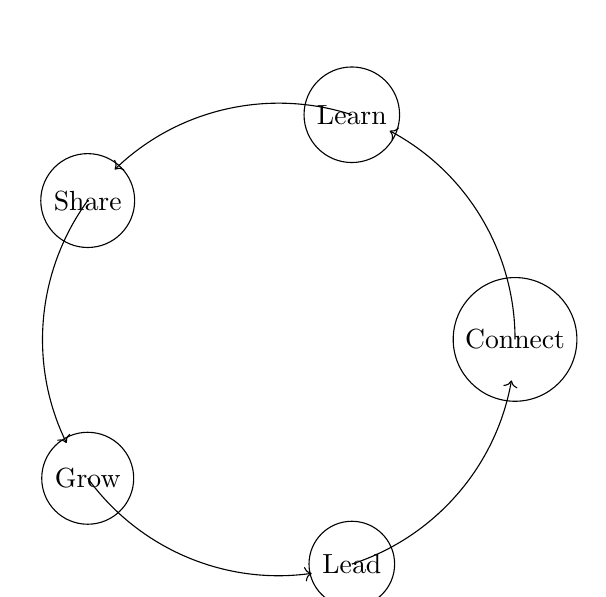
\begin{tikzpicture}
        % Community engagement cycle
        \foreach \angle/\label in {
            0/Connect,
            72/Learn,
            144/Share,
            216/Grow,
            288/Lead
        } {
            \node[draw,circle] at (\angle:3) {\label};
            \draw[->] (\angle:3) arc (\angle:\angle+62:3);
        }
    \end{tikzpicture}
    \caption{Community Engagement Cycle}
\end{figure}


\section{Resource Access Guide}
\begin{tcolorbox}[colback=white,colframe=primary,title=\textbf{Digital Resources}]
    \begin{enumerate}
        \item Document Templates
        \item Market Research
        \item Expert Directory
        \item Event Calendar
        \item Discussion Forums
        \item Knowledge Base
    \end{enumerate}
\end{tcolorbox}


\section{Community Benefits}
\begin{center}
    \begin{tabular}{p{0.3\textwidth}|p{0.6\textwidth}}
        \textbf{Benefit}    & \textbf{Description}                  \\
        \hline
        Expert Access       & Direct connection to industry experts \\
        Resource Library    & Comprehensive template collection     \\
        Market Intelligence & Regular market updates and analysis   \\
        Networking          & Regular virtual and physical events   \\
        Support             & Dedicated community support team      \\
    \end{tabular}
\end{center}

\begin{importantbox}
    Visit circle.counseal.com to activate your membership and access these resources.
\end{importantbox}

\end{document}